\documentclass{article}
\usepackage[top=2cm, bottom=3cm, left=2cm, right=2cm]{geometry}
\usepackage[utf8]{inputenc}
\usepackage{amsmath}
\usepackage{nccmath}
\usepackage{amsfonts}
\usepackage[T1]{fontenc}
\usepackage{makecell}
\usepackage{graphicx}
\usepackage{caption}
\usepackage{subcaption}
\usepackage{minted}
\usepackage{pdfpages}
\usepackage{tabulary}
\usepackage[numbers]{natbib}
\usepackage[colorlinks=true, allcolors=blue]{hyperref}
\renewcommand\theadfont{\bfseries\sffamily}
\usepackage{amssymb}
\usepackage{listings}
\let\oldquote\quote
\let\endoldquote\endquote
\renewenvironment{quote}[2][]
  {\if\relax\detokenize{#1}\relax
     \def\quoteauthor{#2}%
   \else
     \def\quoteauthor{#2~---~#1}%
   \fi
   \oldquote}
  {\par\nobreak\smallskip\hfill(\quoteauthor)%
   \endoldquote\addvspace{\bigskipamount}}



\title{4M21: Software Engineering and Design}
\author{Kazal Oshodi }
\date{January 2023}

\begin{document}

\maketitle
\tableofcontents

\section{Lecture 1 - Software Engineering Introduction}
Software Engineering: a collection of methods,techniques and tools that could be applied to design, build and maintain the instructions for telling a computer what to do and how to do it
\subsection{Software Process}\label{sp}
\begin{itemize}
    \item Analysis: process of understanding the requirements, constraints and goals of a software development project in order to identify the best solution + alignment with stakeholder's needs
    \item Design: creating a definition of how project goals will be achieved
    \item Implementation: process of writing code - normally split into many subprojects
    \item Building: creating a complete version of software - putting all code together + custom configurations for target deployment
    \item Testing: 
    \begin{itemize} 
    \item Unit Tests: making sure that small independent parts of code work correctly 
    \item Integration Tests: all code parts work together
    \item Acceptance: functionality meets requirements
    \item Regression: New code doesn't break old
    \end{itemize}
    \item Deployment: release of software into end user environment
    \item Maintenance: supporting software during its lifetime i.e new software updates
\end{itemize}
Normally, 80-90\% of software system Total Cost Of Ownership (all costs associated with a product over its life cycle) is due to maintenance. This is because the cost of change is high + better to extend existing system to get better return on investment
\subsection{Requirement Analysis}
\begin{quote}{Fred Brooks, "No Silver Bullet - Essence and Accident in Software Engineering"}
    The hardest single part of building a software system is deciding precisely what to build
\end{quote}
It is impossible to know everything in advance required to build a system:
\begin{itemize}
    \item Users don't know 100\% what everything should do
    \item Developers don't know 100\% how users would use it
    \item Only 100\% certainty is that things will change
\end{itemize}
\subsection{Software Engineering Aims}
Software Engineering aims to manage complexity + minimise risks, as well as designing systems that can meet requirements, adapt to changes + withstand any unexpected use cases
\section{Lecture 2 - Object Oriented Programming Design and Analysis}
\subsection{Object Oriented Programming}
"Any computable function" can be achieved by:
\begin{itemize}
    \item "Sequencing" $\rightarrow$ ordered statements
    \item "Selection" $\rightarrow$ conditions, if/else
    \item "Repetition" $\rightarrow$, iterations
\end{itemize}
Object-Oriented Programming: a method of implementation in which programs are organised as cooperative collections of objects. \\ Object-Oriented Design: a method of design encompassing the process of object-oriented decomposition, i.e using objects + classes to describe the system \\
Object-Oriented Analysis: a method of analysis that examines requirements from the perspective of the classes and objectives found in the vocabulary of the problem domain
\subsection{Abstraction}
We can use an object-oriented approach to describe a system in terms of meaningful abstractions (classes), relationship and interactions between them. \\ Abstractions are generalisations that define certain key characteristics and behaviours e.g all cars have 4 wheels. \\ In Object-oriented design, recognising the sameness amongst things can allow us to create abstractions which cause smaller applications and simpler architectures. \\ Abstraction is about: 
\begin{itemize}
    \item Dealing with ideas
    \item Generalisation 
    \begin{itemize}
        \item To focus on what matters - on key characteristics and behaviours
        \item To simplify and make complexity more manageable
    \end{itemize}
\end{itemize}
\subsubsection{Class}
A class encapsulates data and behaviour. When thinking about object-oriented design, need to consider:
\begin{itemize}
    \item What classes of objects are present in the problem?
    \item What behaviour should each class provide?
    \item What should happen when an action is requested of an object?
\end{itemize}
\begin{figure}[H]
\centering
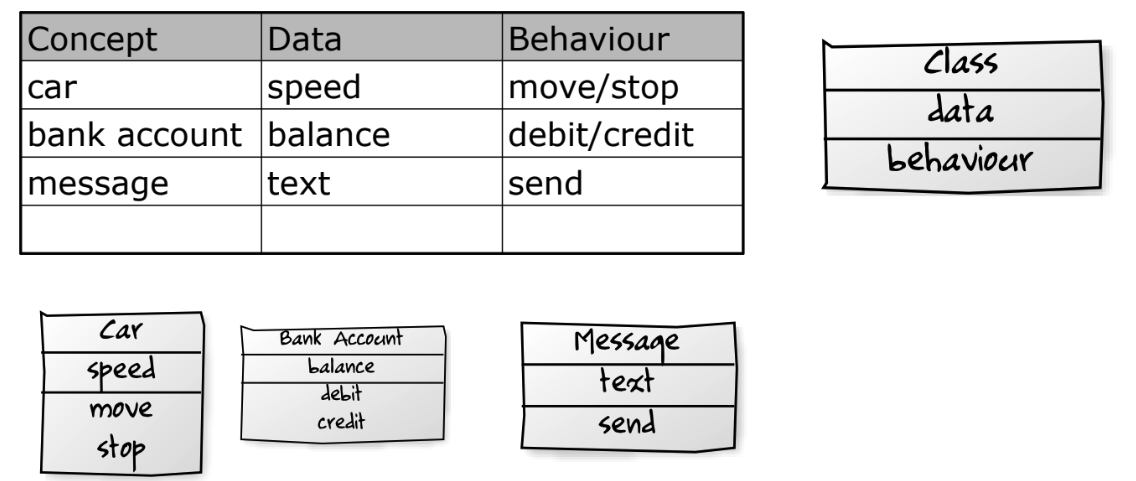
\includegraphics[width = 0.5\linewidth]{Pictures/Screenshot 2023-01-25 at 11.43.59.png}
\caption{Example of classes}
\end{figure}
Note however, that we don't want an abundance of classes. Each class might only be useful for a particular application, and thus should be used for that purpose. For example, a student in the view of the Teaching Office is characterised by the modules they are taking, whereas from the tutor viewpoint they are characterised by their wellbeing.
\subsubsection{Object}
Each class can create multiple instances (objects), which can contain data/behave like the class it is made from. For example the bank account class can be used to create two bank accounts which can credit/debit cash
\begin{figure}[H]
\centering
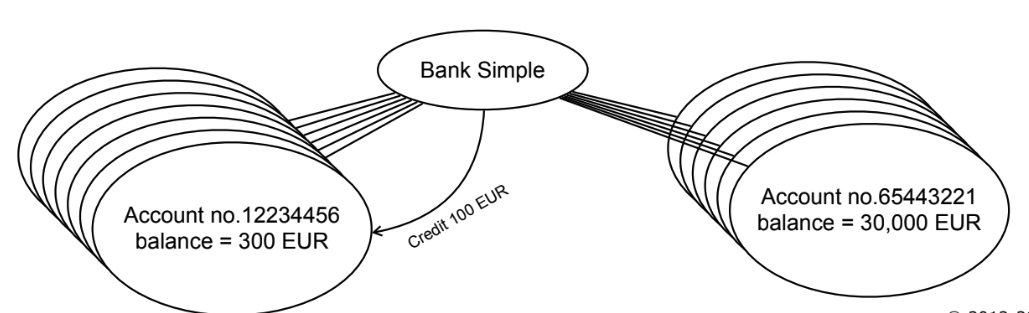
\includegraphics[width = 0.5\linewidth]{Pictures/Screenshot 2023-01-25 at 11.46.39.png}
\caption{Two Objects derived from the same class}
\end{figure}
\subsubsection{Encapsulation}
Classes can provide abstraction. This means that an object can be used without the knowledge of how it works. We want to expose only what it can do and not how, e.g that a steering wheel will make a car turn left if we turn it left, without any knowledge about how this occurs. This is encapsulation \\ \\ Suppose a person has a Name attribute. If we want to access the Name, we could do this directly:
\begin{minted}{Java}
class Person 
{
    public String FIRST_NAME = "John"
    public String LAST_NAME = "Smith"
}
print Person.FIRST_NAME + Person.LAST_NAME
\end{minted}
But, if we wanted to print the last name first e.g in France, then we could:
\begin{minted}{Java}
if (in France)
    print Person.LAST_NAME + Person.FIRST_NAME
else
    print Person.FIRST_NAME + Person.LAST_NAME

\end{minted}
But, it would be easier to keep Name variables hidden (encapsulation), and just use a method to access them instead:
\begin{minted}{Java}
class Person
{
    private String FIRST_NAME = "John"
    private String LAST_NAME = "Smith"

    public String NAME
    {
    if (in France)
        return Person.LAST_NAME + Person.FIRST_NAME
    else 
        return Person.FIRST_NAME + Person.LAST_NAME
    }
}
print Person.NAME
\end{minted}
We use encapsulation to:
\begin{itemize}
    \item Hide implementation
    \item Reduce dependencies between different parts of the application - decoupling
    \item Make changes safely
    \item Debug easier
    \item Make everything more manageable
\end{itemize}
Thus we should try to encapsulate as much as possible.
\subsubsection{Getters/Setters}
We use getters and setters to allow for controlled access to internal data fields.
\begin{minted}{Java}
class Person
{
    private String email;
    public String getEmail {
        return email;
    }
    public setEmail( String newEmail) {
    if ((newEmail != null) && (newEmail.contains('@'))){
        email = newEmail;
    }
    }
}
\end{minted}
We can do this to implement constraint checking, as well as control concurrent access - allowing only one thread to access an object at a time. It also allows for the actual data source to be hidden so it can't be access. \\ \begin{quote}{Martin Fowler}
    The point of encapsulation isn't really about hiding the data, but hiding design decisions, particularly in areas where those decisions may have to change. 
\end{quote}
For example, if you want to communicate with an external data source, use encapsulation, because we want to focus on the messages delivered to the data source rather than the data source itself. \\ If we don't have controlled access to internal data fields, then this means that:
\begin{itemize}
    \item We can't abstract the class
    \item We can't remove/reduce dependencies between different parts of the system
    \item We can't make changes safely
    \item We can't debug quickly
\end{itemize}
Thus, we should hide everything except what we want to expose.
\subsection{Inheritance}
Classes can be related: 
\begin{itemize}
    \item Superclass/base class (parent) can be extended/inherited from
    \item Subclass (child) extends/inherits from superclass
\end{itemize}
Each subclass can do everything a superclass can, but they can also:
\begin{itemize}
    \item Hold additional data
    \item Perform new actions
    \item Perform original actions differently
\end{itemize}
For example with a shape:
\begin{figure}[H]
\centering
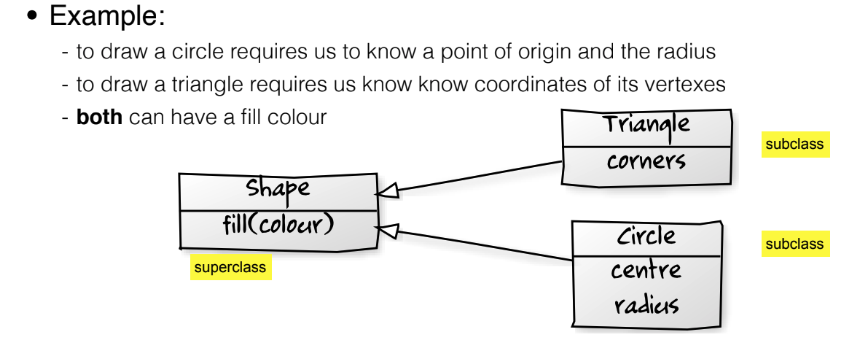
\includegraphics[width = 0.5\linewidth]{Pictures/Screenshot 2023-01-25 at 13.26.24.png}
\caption{Inheritance}
\end{figure}
\subsection{Polymorphism}
Polymorphism allows us to request the same action from objects, but execute it in different ways. For example, if we have different bank accounts, but we want to find out how much money is in each account, then the action is the same - request the current balance. However, the way the balance could be calculated could be different. But we can still use polymorphism to simplify our code. This is an example of class inheritance hierarchy, which lets us choose the level of abstraction at which we interact with an object. \\ For example, compare this code:
\begin{minted}{Java}
for CurrentAccount in Bank 
{
    TotalMoney += CurrentAccount.balance()
}
for SavingAccount in Bank 
{
    TotalMoney += SavingAccount.balance()
}
for SuperHighInterestAccount in Bank 
{
    TotalMoney += SuperHighInterestAccount.balance()
}
\end{minted}
To this code:
\begin{minted}{Java}
for Account in Bank
{
    TotalMoney += Account.balance()
}
\end{minted}
\begin{figure}[H]
\centering
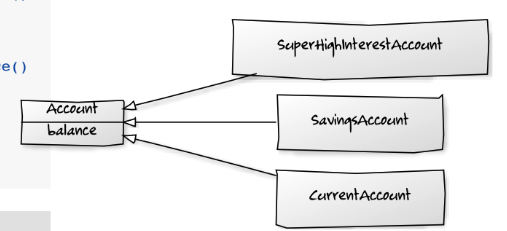
\includegraphics[width = 0.5\linewidth]{Pictures/Screenshot 2023-01-25 at 13.33.03.png}
\caption{Polymorphism}
\end{figure}
Polymorphism seperates the declaration of functionality from the specifics of its implementation.
\subsection{Identifying good Classes}
Remember: Inheritance "IS A" Relationship - Subclass "IS A" Superclass i.e Coffee IS A Drink, Car IS A Vehicle
\begin{figure}[H]
\centering
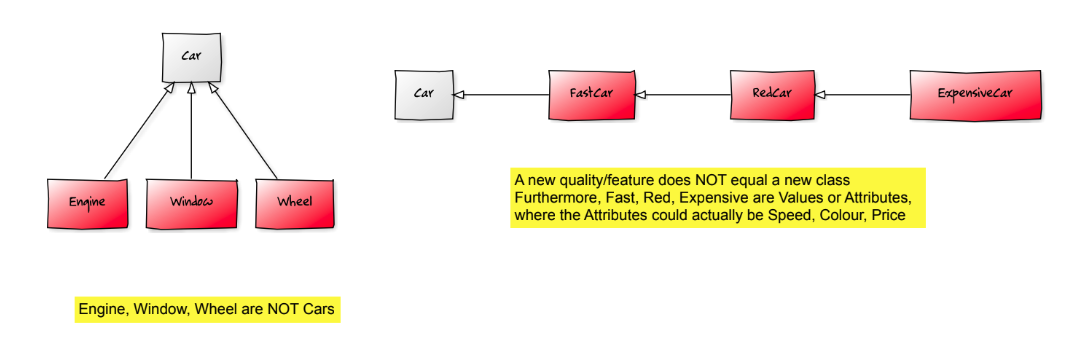
\includegraphics[width = 0.8\linewidth]{Pictures/Screenshot 2023-01-25 at 13.36.04.png}
\caption{Bad Classes}
\end{figure}
\subsection{Abstract Classes}
We want our classes to be abstract - a class which can't be instantiated. This means that we can't define the class without going into more detail. This is good for capturing the higher level view of a system
\begin{figure}[H]
\centering
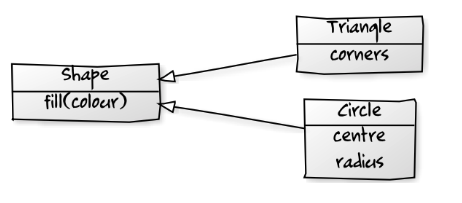
\includegraphics[width = 0.5\linewidth]{Pictures/Screenshot 2023-01-25 at 13.37.34.png}
\caption{Abstract Class}
\end{figure}
\subsection{Interfaces}\label{interface}
An interface is a purely abstract class which defines only behaviour - not data. This is a point where two entities meet and interact. It defines a set of ways to interact with a class, or a contract of what must be avaliable. Interfaces help to add specific behaviour to classes. Most classes with extend one superclass, but will implement multiple interfaces.
\begin{figure}[H]
\centering
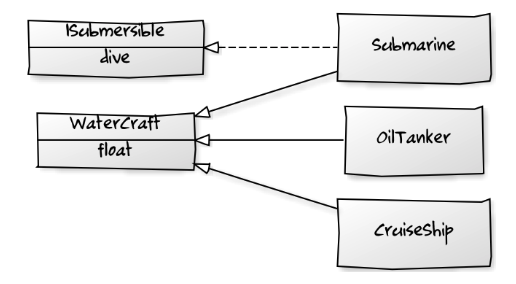
\includegraphics[width = 0.5\linewidth]{Pictures/Screenshot 2023-01-25 at 13.39.41.png}
\caption{Interfaces}
\end{figure}
\pagebreak
\section{Lecture 3 -Introduction to UML}
UML is a formal graphical language which has a set of diagrams for describing software systems. This can be used for designing, documenting and communicating software architecture + program behaviour. \\
There are 14 types of diagrams defined:
\begin{figure}[H]
\centering
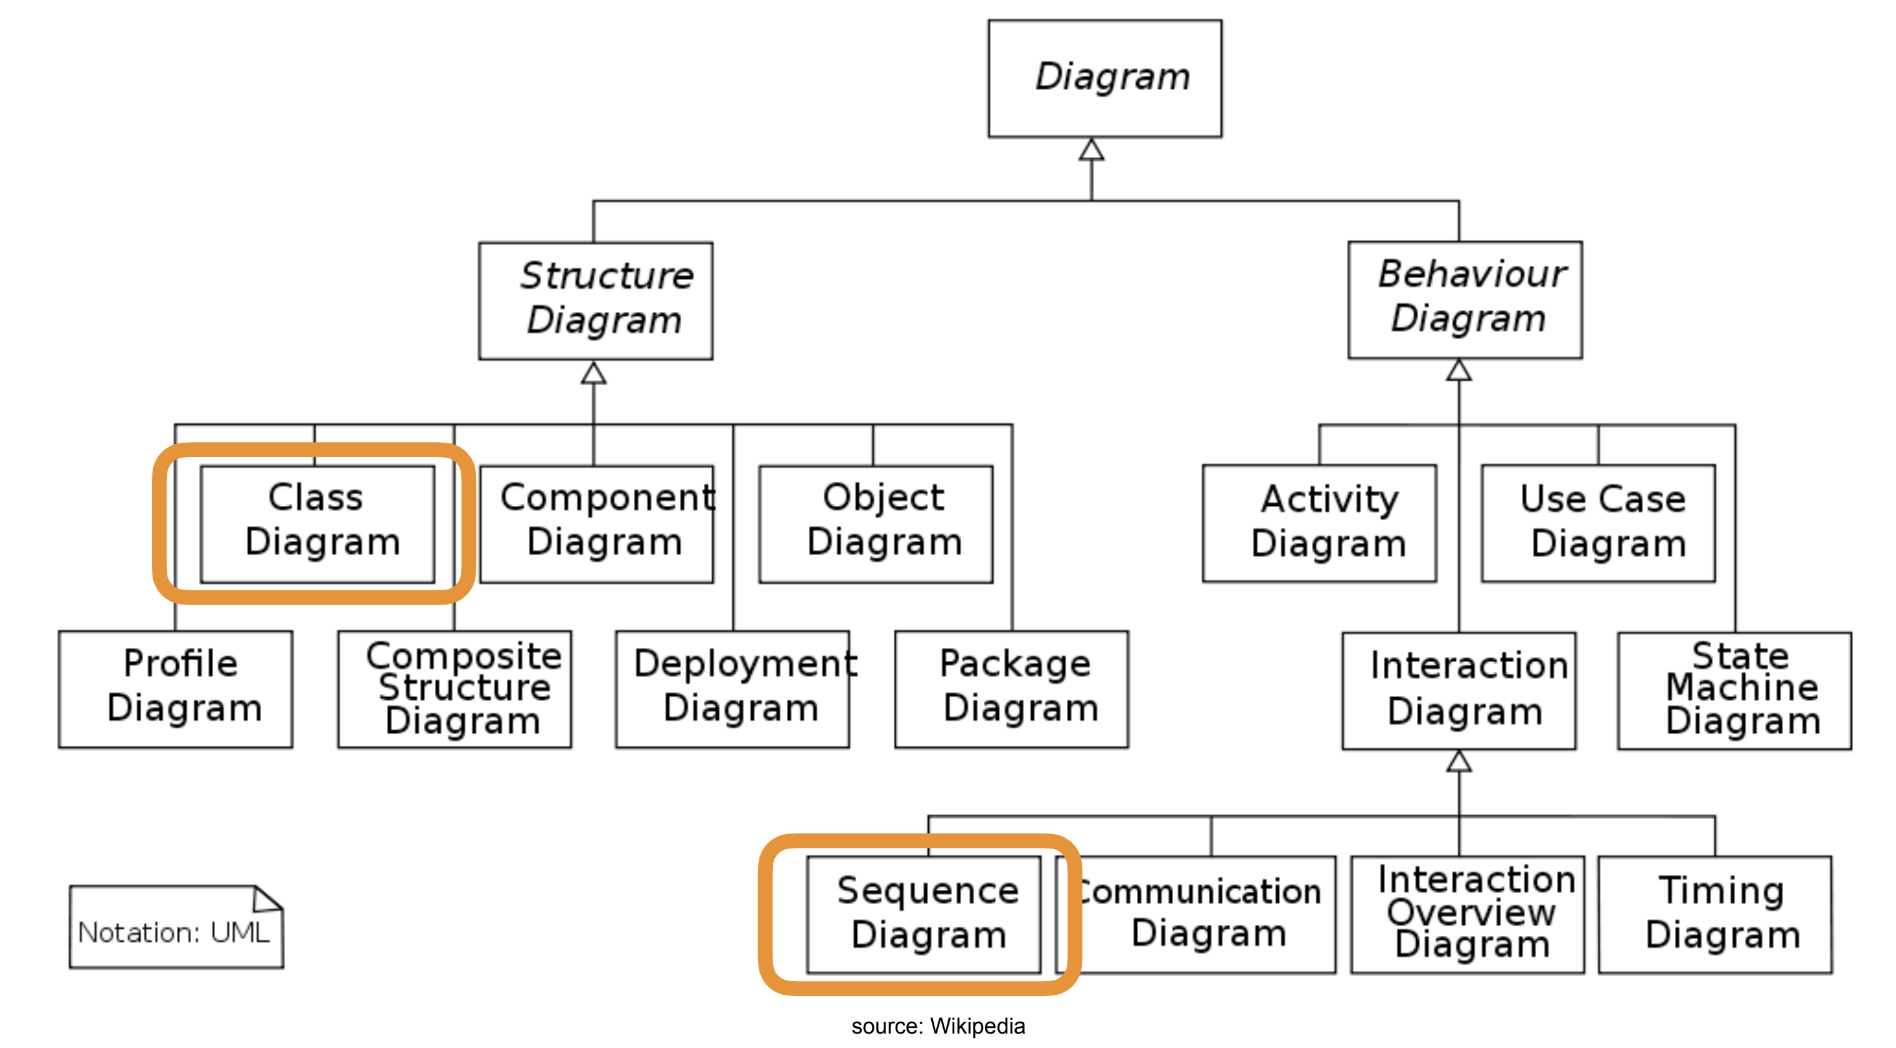
\includegraphics[width = 0.5\linewidth]{Pictures/Screenshot 2023-01-27 at 12.04.06.png}
\caption{UML Types}
\end{figure}
To describe a system we need:
\begin{itemize}
    \item Structures: Items + how they are connected
    \item Behaviour: How items interact
\end{itemize}
UML, we use Class Diagrams to represent structures. These describe the software architecture by explaining what classes are in a system + their relationships. \\
Behaviour diagrams such as Sequence and Communication Diagrams show interaction between objects. \\
We want to use UMLAsSketch to communicate parts of the system to a group of people.
\subsection{Class Diagram}
These show the classes in a software system, along with their attributes, operations and relationships:
\begin{figure}[H]
\centering
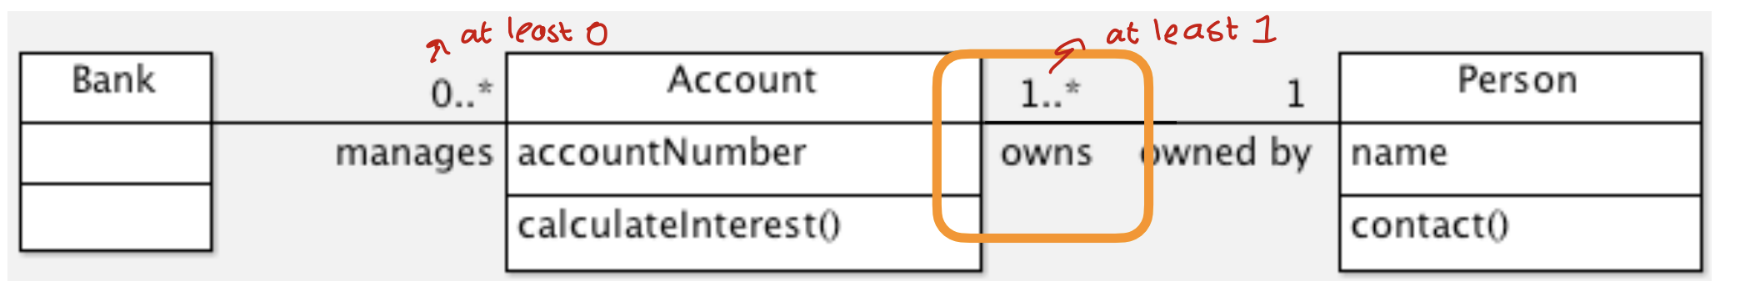
\includegraphics[width = 0.8\linewidth]{Pictures/Screenshot 2023-01-27 at 12.09.45.png}
\end{figure}
Explaining this diagram: 
\begin{itemize}
    \item Bank can manage at least 0 accounts
    \item An Account has an account number and can calculate interest
    \item Each Account can be owned by one Person
    \item One Person can own multiple accounts
    \item Each Person has a name and can be contacted
\end{itemize}
Each class is represented by 3 different sections: name, attributes and operations/methods:
\begin{figure}[H]
\centering
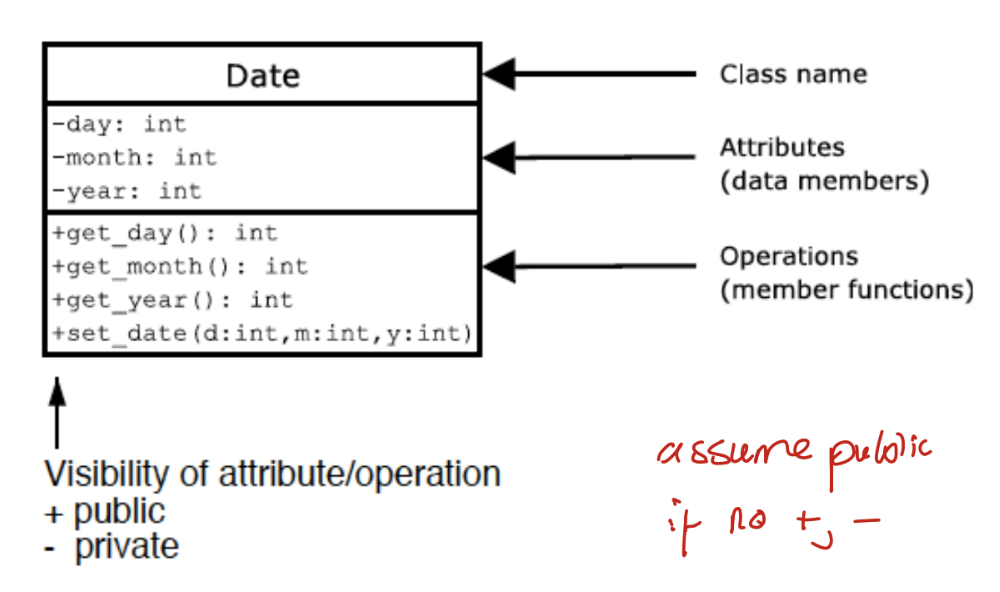
\includegraphics[width = 0.6\linewidth]{Pictures/Screenshot 2023-01-27 at 12.12.02.png}
\end{figure}
We try to only include public features of a class in UML as they can be used in relation with other classes.
\begin{figure}[H]
\centering
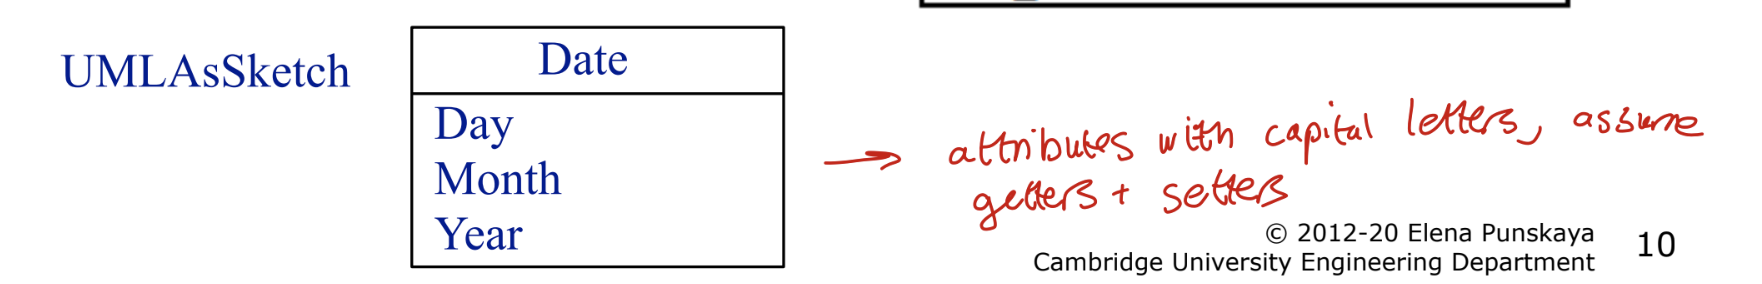
\includegraphics[width = 0.6\linewidth]{Pictures/Screenshot 2023-01-27 at 12.13.24.png}
\end{figure}
We want to have the right level of abstraction to keep the diagrams concise and useful:
\begin{figure}[H]
\centering
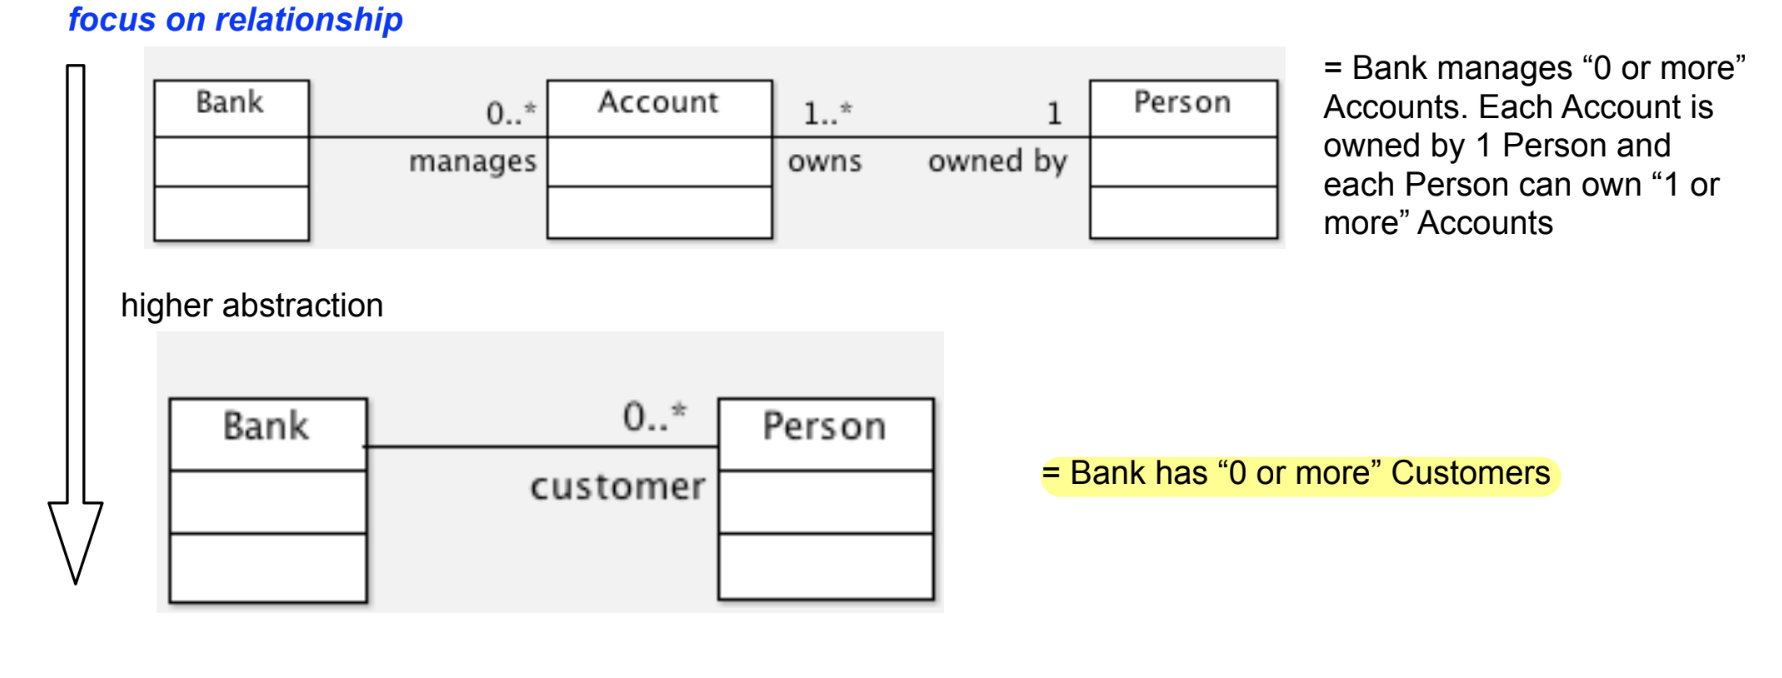
\includegraphics[width = 0.6\linewidth]{Pictures/Screenshot 2023-01-27 at 12.16.58.png}
\end{figure}
At some points, might be best to get rid of all methods and attributes to just focus on relationships.
\subsection{Association}
In class box, we represent attributes as a line of text i.e a reference to a Time Object:
\begin{figure}[H]
\centering
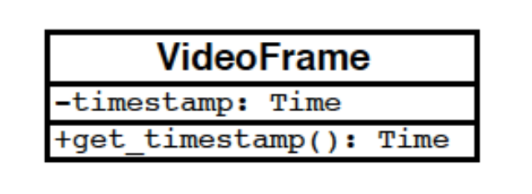
\includegraphics[width = 0.3\linewidth]{Pictures/Screenshot 2023-01-27 at 12.18.38.png}
\end{figure}
But, we can also show that using association, with a solid line with an arrow. This indicates that the class uses an attribute of that object. This is mostly used for more significant classes.
\begin{figure}[H]
\centering
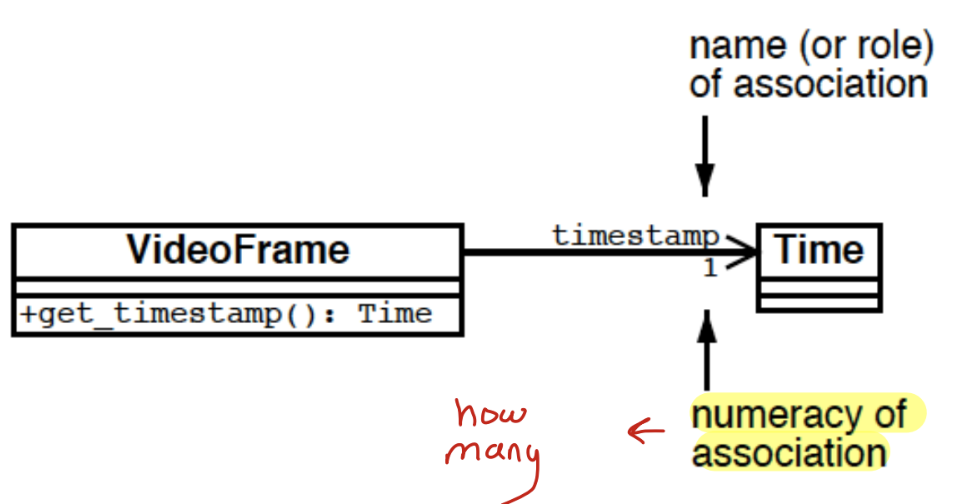
\includegraphics[width = 0.6\linewidth]{Pictures/Screenshot 2023-01-27 at 12.20.22.png}
\end{figure}
This line is:
\begin{itemize}
    \item Directional - unidirectional association
    \item Meaningful - need to name what the attribute is defined as in the class
    \item Constrained - it is stated how many Time objects a VideoFrame can be in this relationship at the same time i.e 1. This can also be a range e.g 0..1, * (infinite amount) or 1..* (at least 1)
\end{itemize}
\subsection{Navigability}
These associations can also do bidirectional navigability, as seen below.
\begin{figure}[H]
\centering
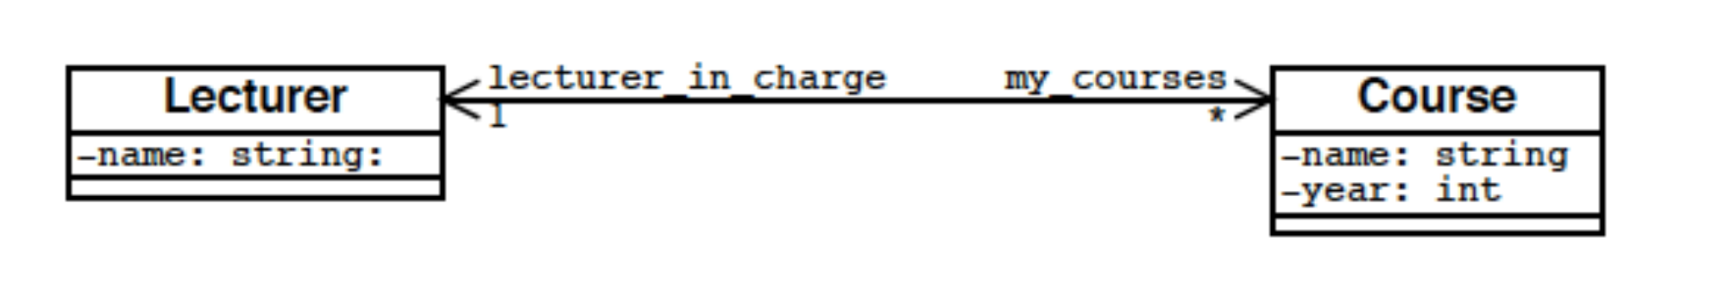
\includegraphics[width = 0.6\linewidth]{Pictures/Screenshot 2023-01-27 at 12.23.32.png}
\end{figure}
From this we can see that each Lecturer object knows about all the courses they are teaching, and * indicates that they can be in charge of any number of courses. For each Course, there is only 1 lecture in charge. \\
We might not show the directional of associations if it is not relevant to the meaning of the diagram.
\subsection{Composition - don't need to draw this in exam}
We can include a diamond when having class association. A filled diamond indicates composition
\begin{figure}[H]
\centering
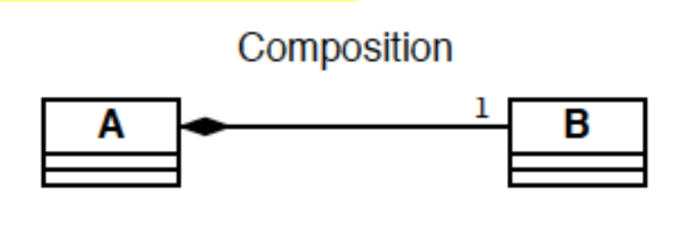
\includegraphics[width = 0.3\linewidth]{Pictures/Screenshot 2023-01-27 at 12.27.25.png}
\end{figure}
This means that if A is destroyed, then B will be destroyed too. These are good to show the strength of relationship between classes i.e exclusive ownership.
\subsection{Aggregation - don't need to draw this in exam}
An empty diamond means objects of class A contain objects of class B. But A doesn't control the lifecycle of B i.e destroying A doesn't destroy B. \\
For example, a college society has students, but closing the society won't destroy the students.
\begin{figure}[H]
\centering
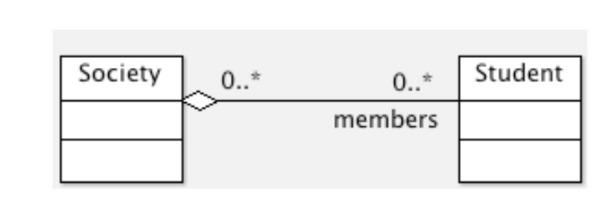
\includegraphics[width = 0.6\linewidth]{Pictures/Screenshot 2023-01-27 at 12.30.49.png}
\end{figure}
\subsection{Inheritance}
We can represent inheritance between classes as:
\begin{figure}[H]
\centering
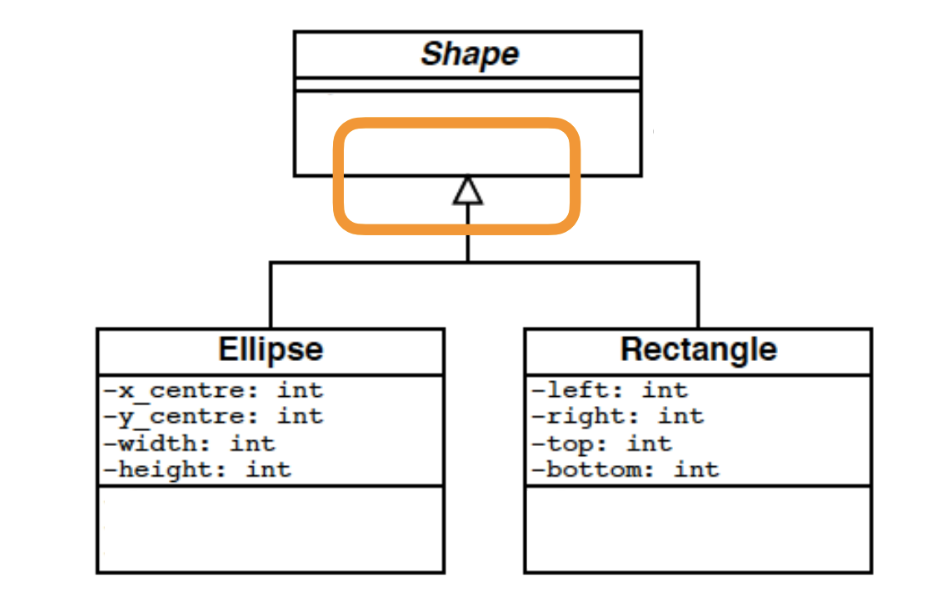
\includegraphics[width = 0.5\linewidth]{Pictures/Screenshot 2023-01-27 at 12.32.13.png}
\end{figure}
\subsection{Abstract Methods}
We can include abstract classes and methods in UML using italics. This can be hard to do in handwriting, so instead, can mark a class/method as \{abstract\}. If a class has an abstract method, then it must be declared as an abstract class.
\begin{figure}[H]
\centering
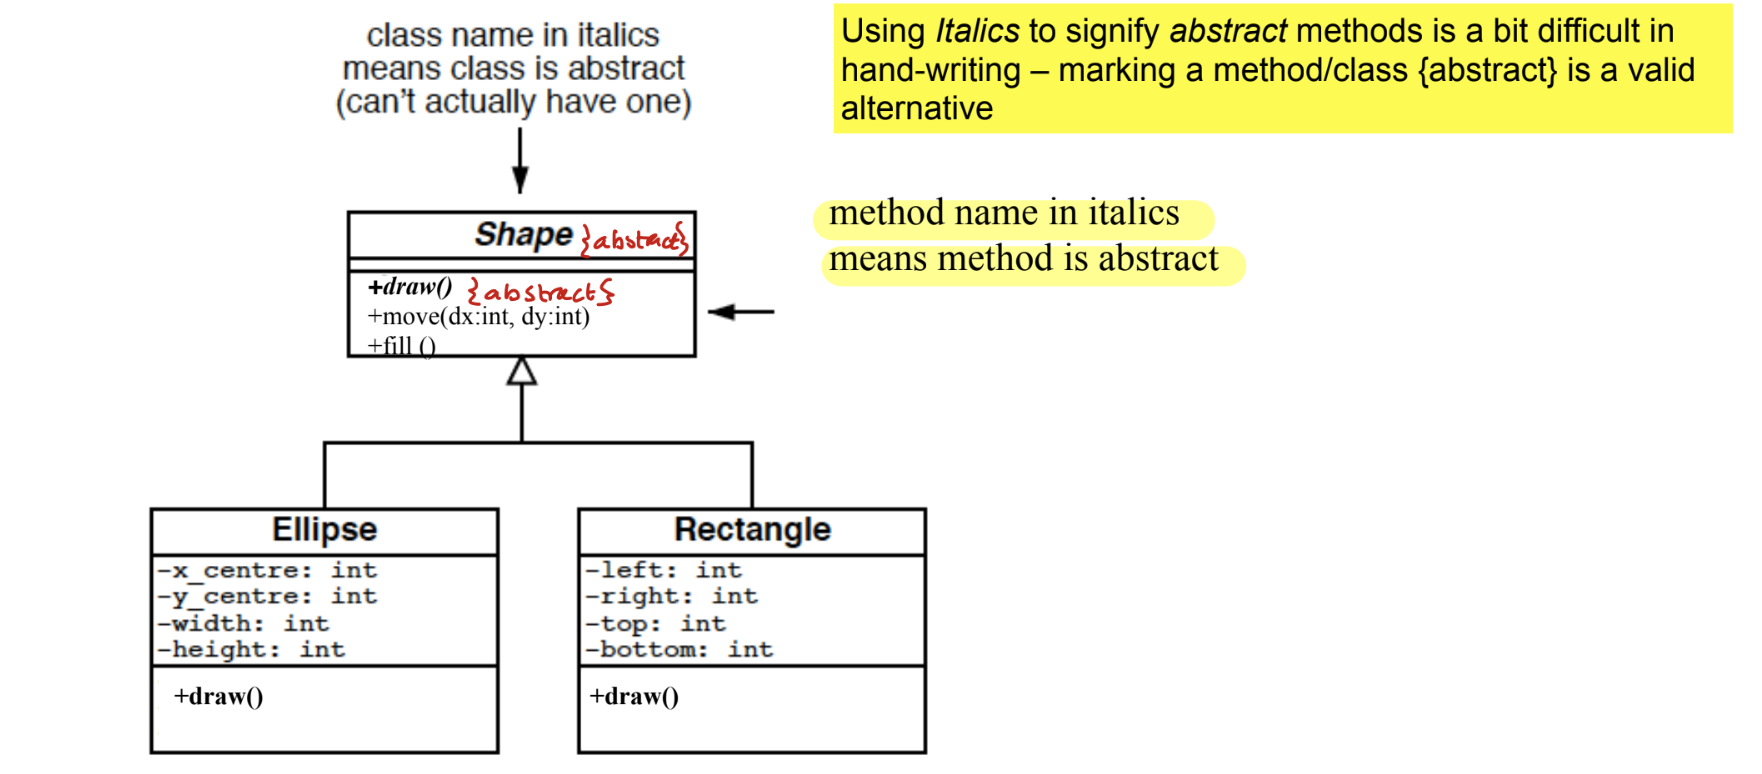
\includegraphics[width = 0.6\linewidth]{Pictures/Screenshot 2023-01-27 at 12.34.03.png}
\end{figure}
\subsection{Interfaces}
Inheritance is useful when:
\begin{itemize}
    \item Implementation inheritance - superclass implements some functionality which can be re-used by all subclasses
    \item Behaviour inheritance - class can expose a certain set of functionality
\end{itemize}
We can use interfaces for methods which might be access by different subclasses, as seen in \hyperref[interface]{Interfaces}. 
\begin{figure}[H]
\centering
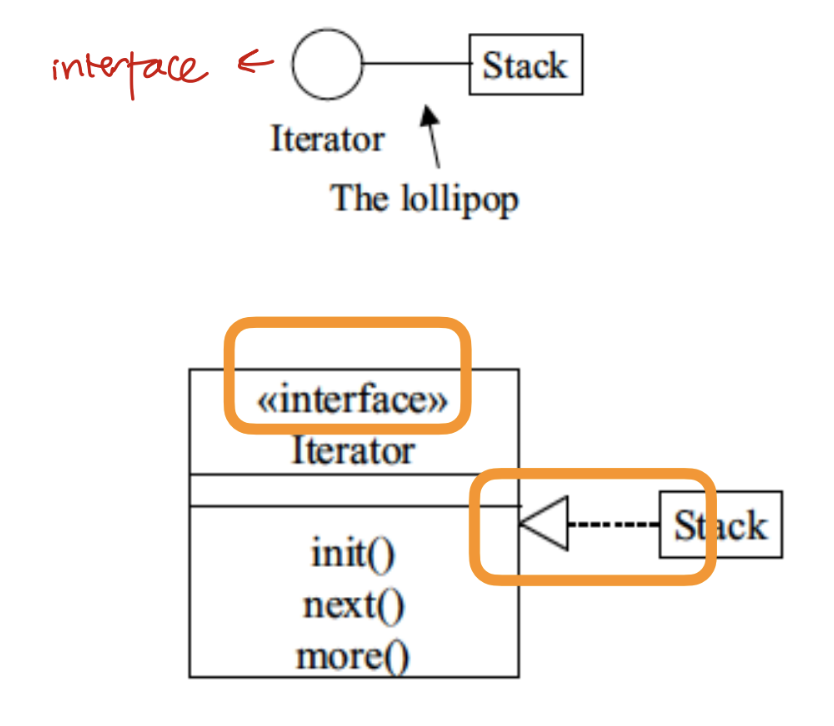
\includegraphics[width = 0.5\linewidth]{Pictures/Screenshot 2023-01-27 at 12.38.37.png}
\caption{UML Interface}
\end{figure}
It is also common to start interface names with the letter I. Interfaces are great to apply the same functionality to very different concepts, like comparing apples to oranges.
\begin{figure}[H]
\centering
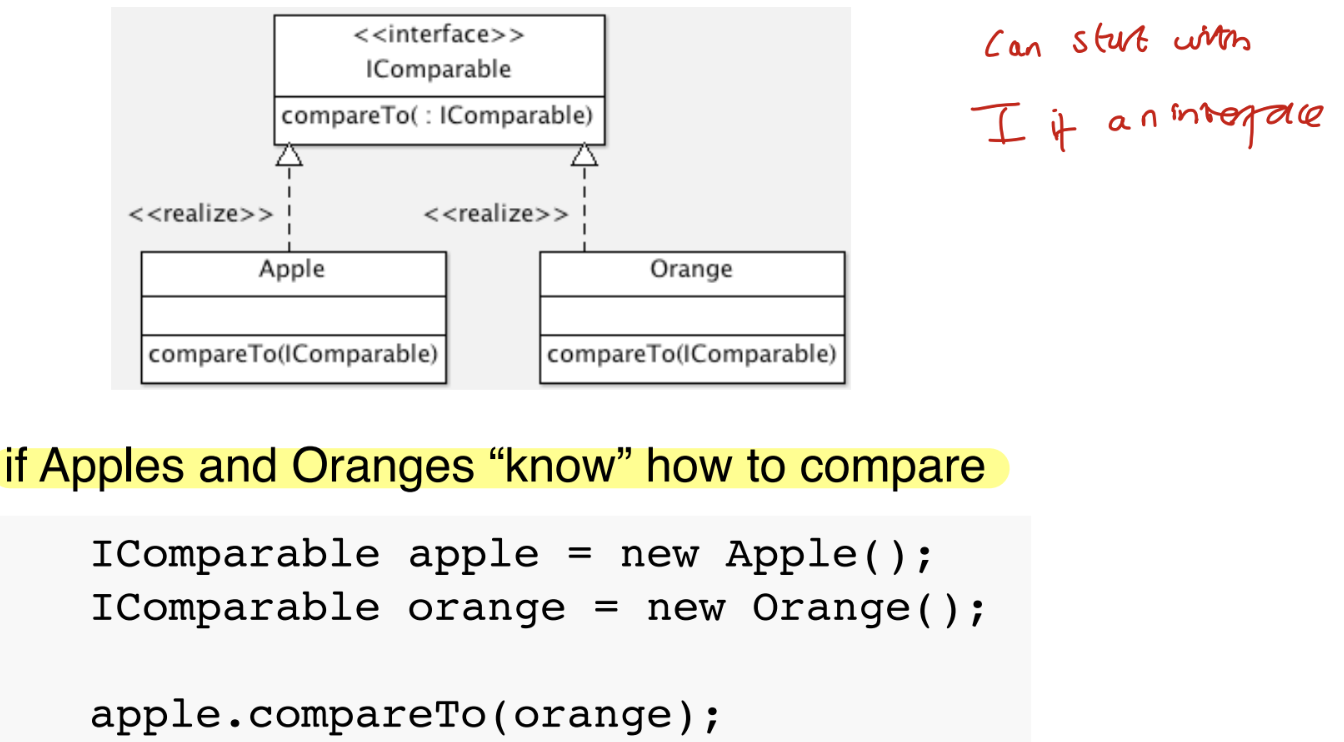
\includegraphics[width = 0.6\linewidth]{Pictures/Screenshot 2023-01-27 at 12.40.28.png}
\end{figure}
\subsection{Class Diagram Example}
\begin{figure}[H]
\centering
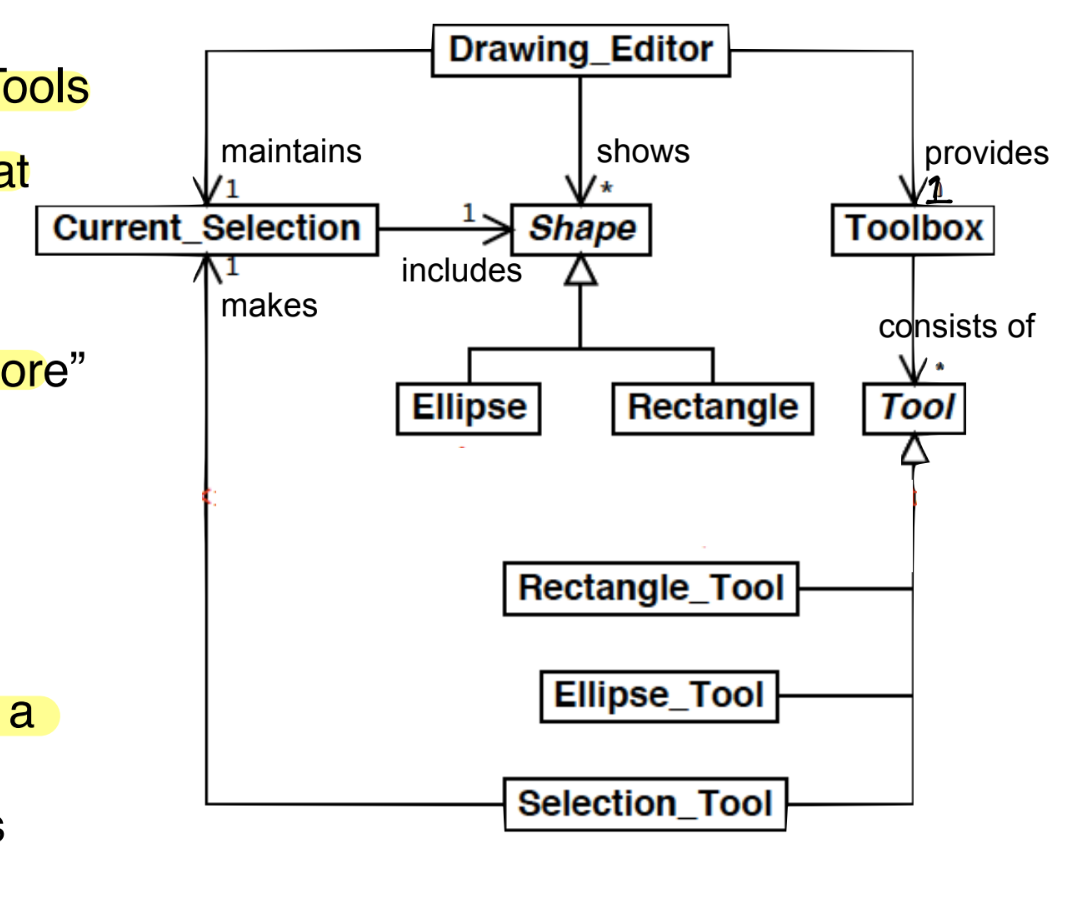
\includegraphics[width = 0.5\linewidth]{Pictures/Screenshot 2023-01-27 at 12.41.28.png}
\caption{Drawing Editor Class}
\end{figure}
Explaining this diagram:
\begin{itemize}
    \item Drawing Editor has 1 Toolbox
    \item Toolbox has any number of Tools
    \item There are 3 types of Tools: Rectangles, Ellipses and make a Selection
    \item The Drawing Editor can show any number of shapes
    \item There are 2 types of shapes: Ellipses and Rectangles
    \item Drawing Editor maintains the current Selection
    \item Only 1 shape can be selected at once
\end{itemize}
\subsection{Dynamic View}
Class Diagrams are good for capturing the relationships, but we need to use dynamic diagrams to show how objects interact with each other for a particular action. There are 2 choices:
\begin{itemize}
    \item Sequence diagrams - they present a more clear view of the timeline. They are easier to read when there are a few objects, with a lot of calls.
    \item Communication diagrams - they focus more on the nature of collaboration between the object to perform an action. They are better if there are a few method calls between many objects.
\end{itemize}
To look at both of them, we can use a drawing editor example:
\begin{figure}[H]
\centering
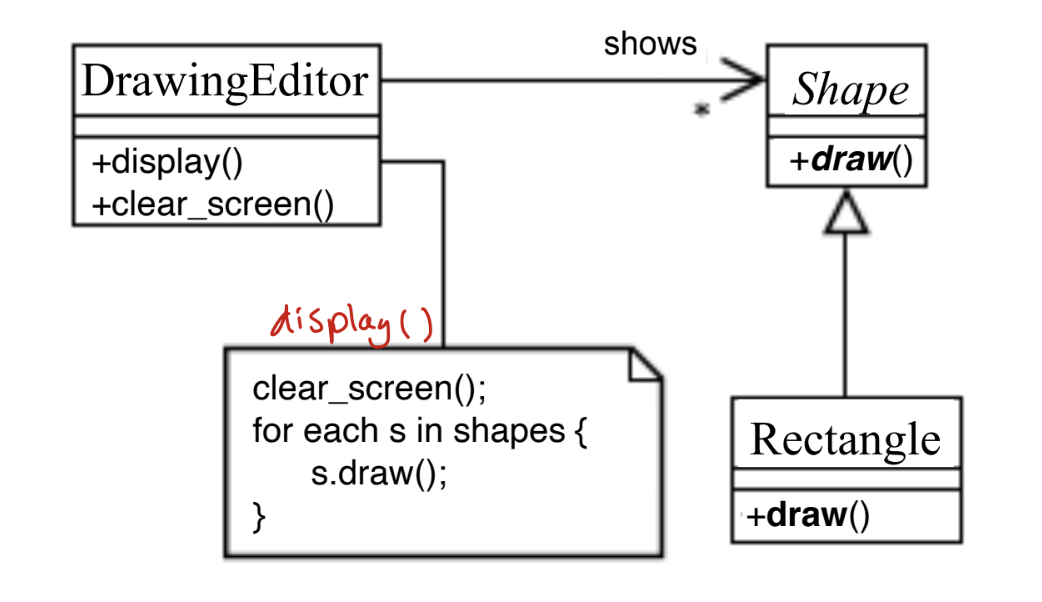
\includegraphics[width = 0.5\linewidth]{Pictures/Screenshot 2023-01-27 at 12.46.49.png}
\end{figure}
If we call the display() method, then we can look at each diagram and how it works:
\subsection{Sequence Diagram}
A Sequence diagram has a vertical axis, representing time, and white boxes to show the duration of each call.
\begin{figure}[H]
\centering
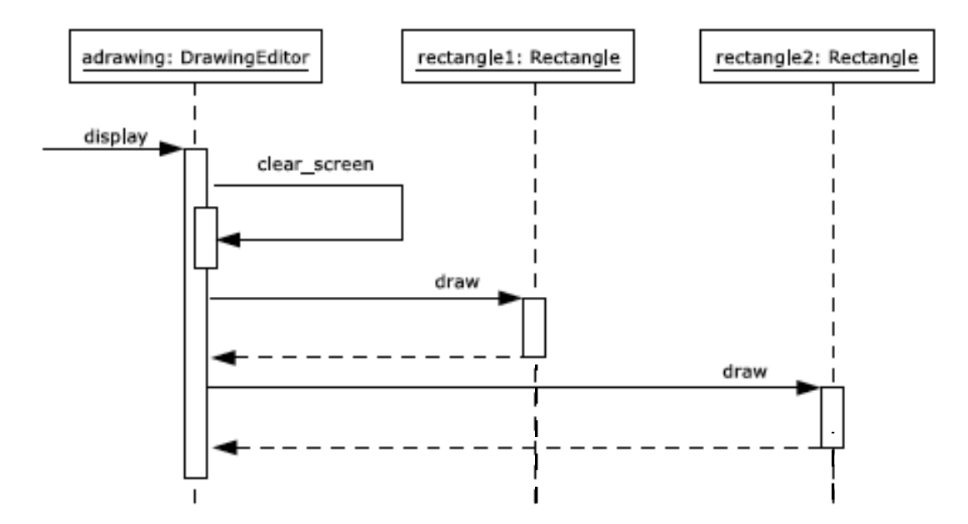
\includegraphics[width = 0.6\linewidth]{Pictures/Screenshot 2023-01-27 at 12.48.22.png}
\caption{Sequence Diagram}
\end{figure}
This works by:
\begin{itemize}
    \item display() is called in adrawing
    \item adrawing calls the clear\_screen() method on itself
    \item adrawing calls the draw() method in rectangle1, which returns
    \item adrawing calls the draw() method in rectangle2, which returns
    \item the display() method is completed
\end{itemize}
We don't always need to include the return from the draw() class (in dashed lines).
\subsection{Communication Diagram}
These show the method flow between objects, by numbering method calls:
\begin{figure}[H]
\centering
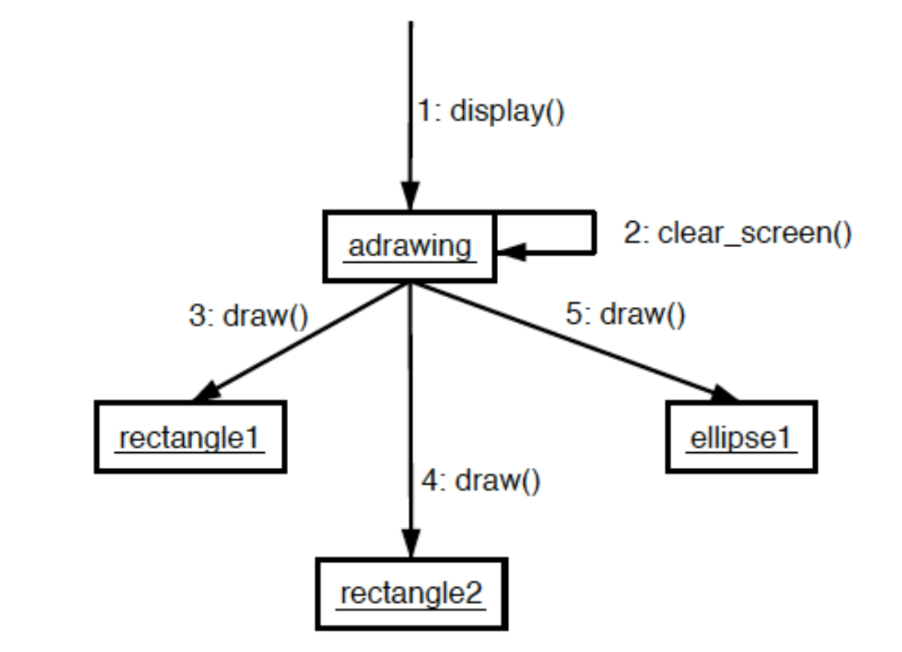
\includegraphics[width = 0.5\linewidth]{Pictures/Screenshot 2023-01-27 at 12.51.42.png}
\caption{Communication Diagram}
\end{figure}
\subsection{State Diagrams}
If the behaviour of an object depends on its state e.g in embedded software, then we can use UML State Diagrams to show it
\begin{figure}[H]
\centering
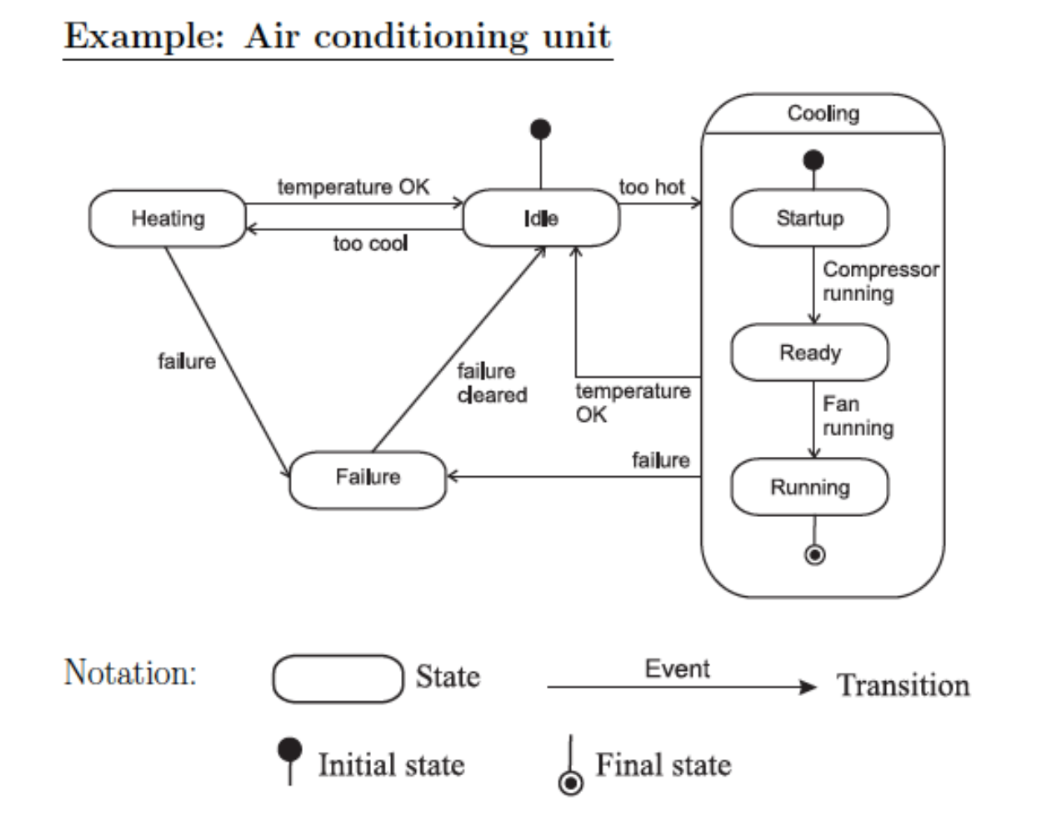
\includegraphics[width = 0.5\linewidth]{Pictures/Screenshot 2023-01-27 at 12.52.49.png}
\caption{State Diagram}
\end{figure}
\subsection{New Notation}
Project Teams can expand UML to their own needs, as long as everyone on the project can understand it, and everyone's understanding is the same
\begin{figure}[H]
\centering
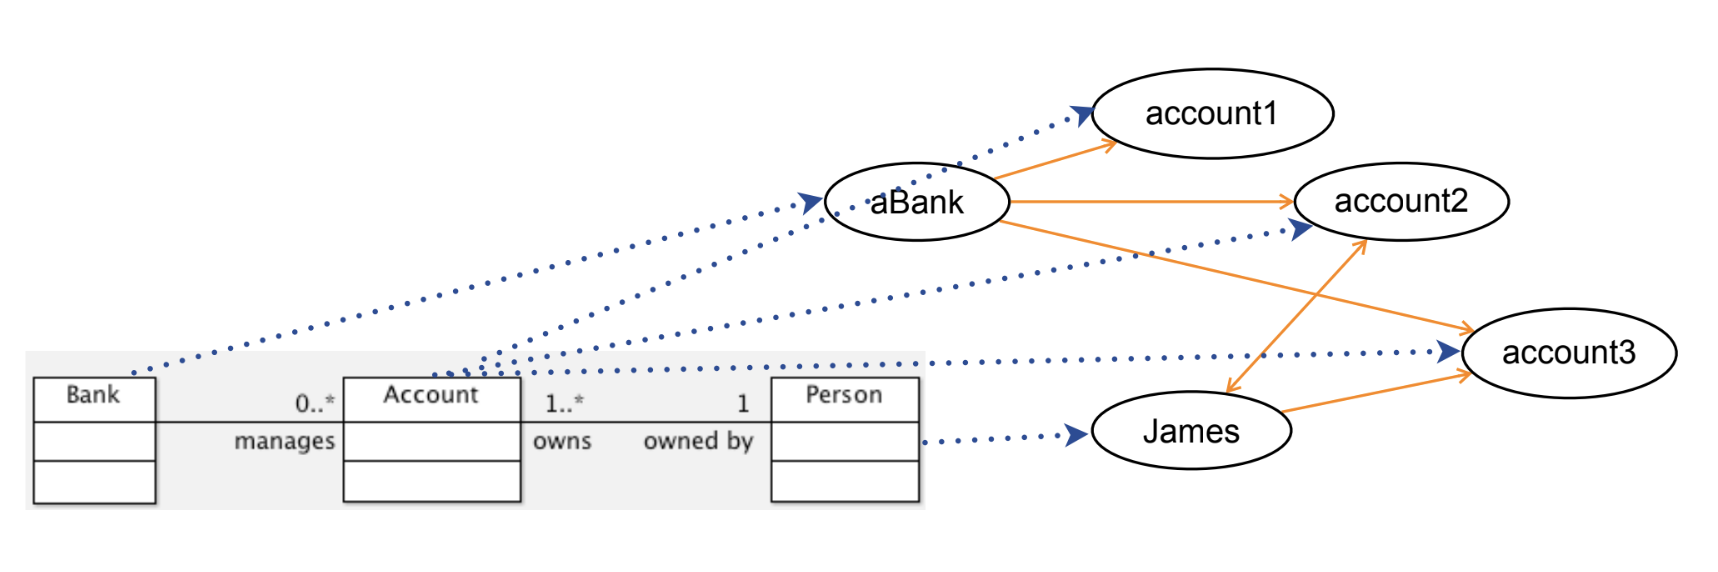
\includegraphics[width = 0.6\linewidth]{Pictures/Screenshot 2023-01-27 at 12.54.30.png}
\end{figure}
\section{Lecture 4 - UML Example}
\subsection*{Library Management System}
Requirements: (\textbf{bold} are the key words)
\begin{enumerate}
    \item \label{req1} Any library member should be able to \textbf{search books} by their \textbf{title, author} or \textbf{subject}
    \item \label{req2} Each book should have a: 
    \begin{itemize}
        \item \textbf{Barcode}
        \item \textbf{Bookshelf number}
        \\ This is to help locate it
    \end{itemize}
    \item \label{req3} A library member can use the library system to \textbf{checkout a copy of a book} using this \textbf{account details} from this library cover and \textbf{barcode} printed on the book
\end{enumerate}
An example class diagram for \eqref{req1}, \eqref{req2}:
\begin{figure}[H]
    \centering
    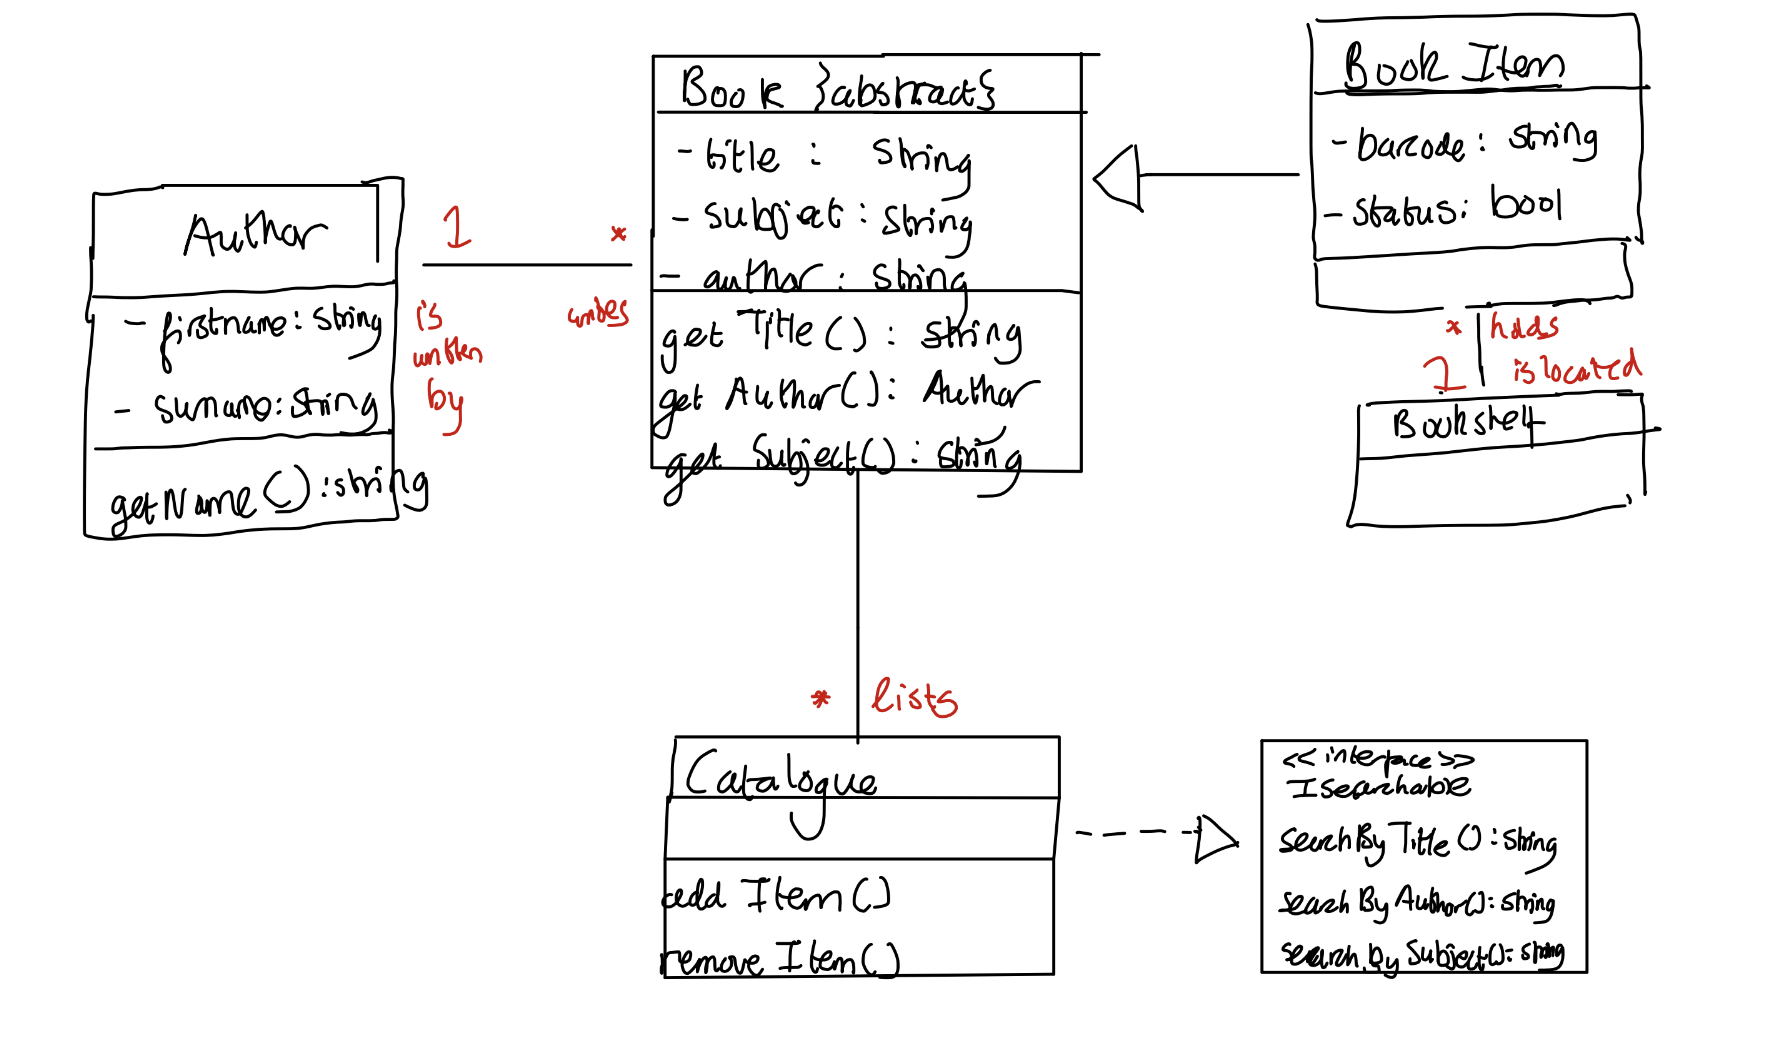
\includegraphics[width = 0.7\linewidth]{Pictures/Screenshot 2023-02-01 at 11.54.43.png}
    \caption{Class Diagram}
\end{figure}
An example sequence diagram for \eqref{req3}:
\begin{figure}[H]
    \centering
    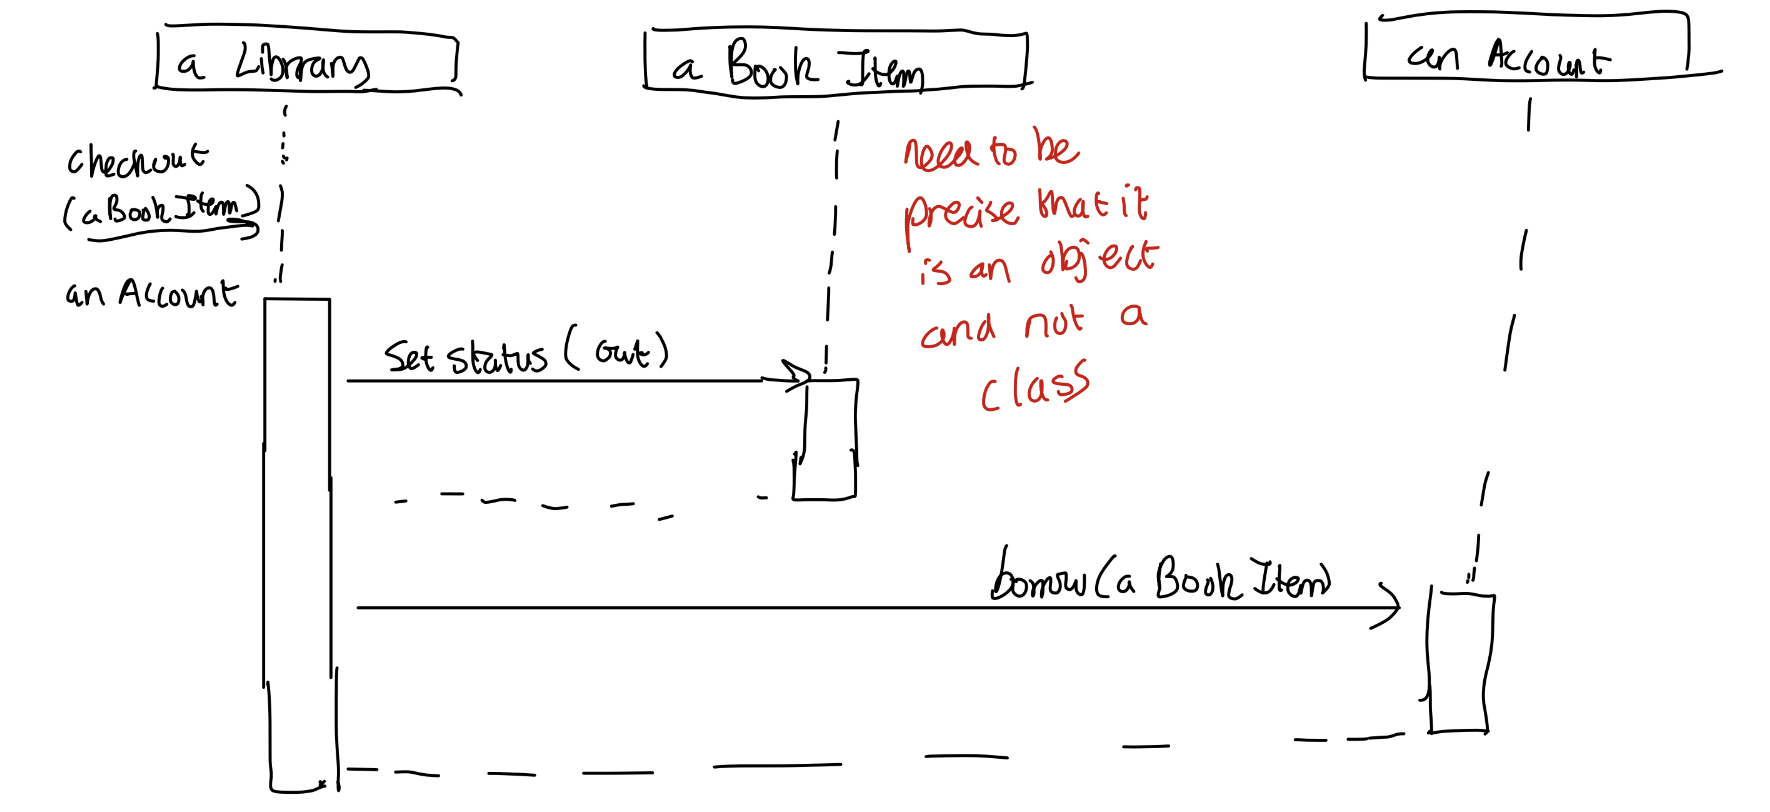
\includegraphics[width = 0.7\linewidth]{Pictures/Screenshot 2023-02-01 at 11.57.39.png}
    \caption{Sequence Diagram}    
\end{figure}
We can include another class diagram for this sequence diagram:
\begin{figure}[H]
    \centering
    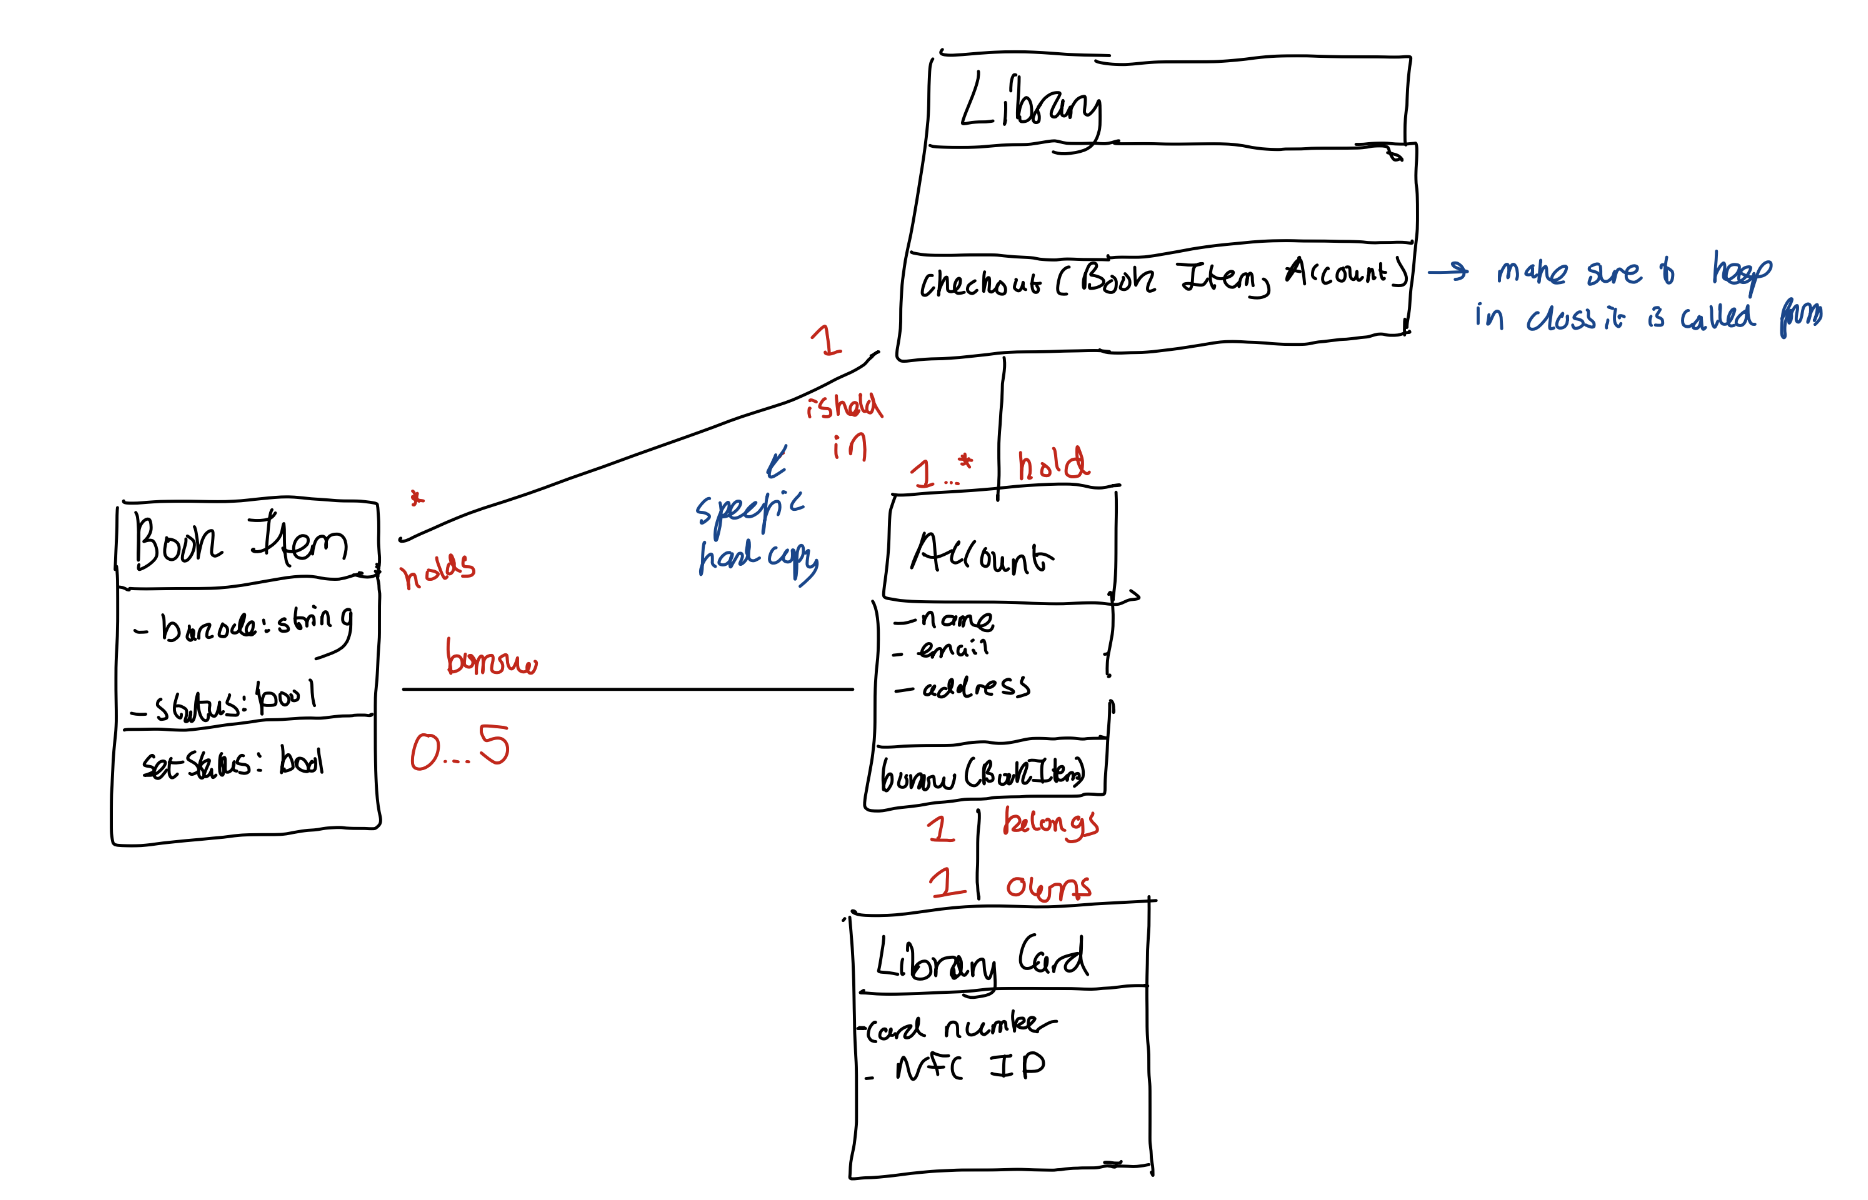
\includegraphics[width = 0.7\linewidth]{Pictures/Screenshot 2023-02-01 at 12.00.26.png}
    \caption{Class Diagram}    
\end{figure}
\section{Lecture 5 - Design Patterns}
We use Design Patterns as the same architectural structures occur in response to commonly occurring problems
\subsection{Structure of Problems}
Each pattern has a standard format:
\begin{itemize}
    \item Motivation: specific functionality we want our software to provide
    \item Solution options: Explore some ways of providing this functionality, and discuss their limitations
    \item Optimal Solution: Present a preferred solution based on a design pattern
    \item Code Example: Give an example of the code of a design solution 
    \item Design Pattern: Discuss the principle underlying a good solution + applicability to other solutions. Can show generic design pattern using UML
    \item Disadvantages: Discuss shortcoming of design pattern, and why you might not want to use it for certain cases
\end{itemize}
\subsection{Composite}
We use the composite design pattern when we want to operate on individual items, and groups of those in a common way. For example, if we want to move folders and files the same way. \\
\subsubsection*{Motivation}
We want our drawing editor to support grouping and ungrouping operations, so that a number of shapes can be collected together and treated as a single entity.
\subsubsection*{Solution Options}
We could add a group member field into Shape to indicate which group each shape belongs to:
\begin{figure}[H]
    \centering
    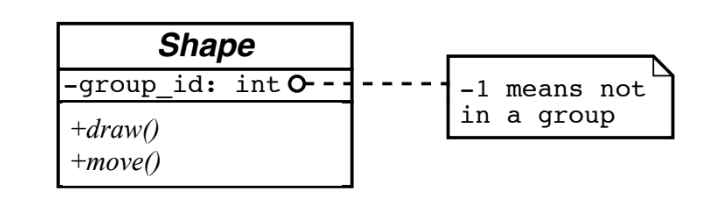
\includegraphics[width=0.6\linewidth]{Pictures/Screenshot 2023-02-05 at 12.27.22.png}
\end{figure}
Pros of this - simple to implement. Cons - can't support nested group
\subsubsection*{Optimal Solution}
We can introduce a new class ShapeGroup to manage a group of shapes. This would be a subclass of Shape, and thus keeps the Shape class interface
\begin{figure}[H]
    \centering
    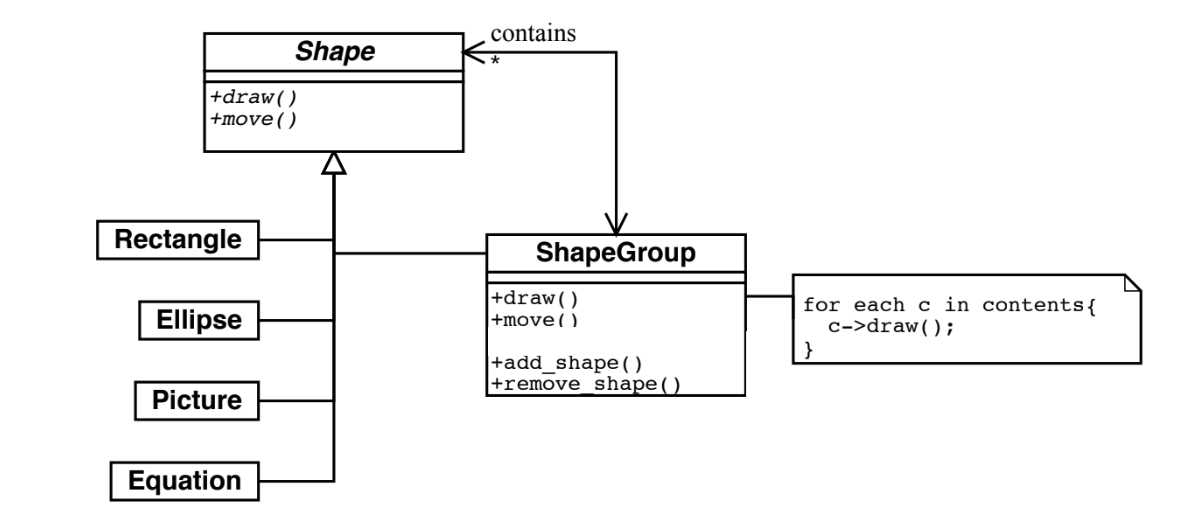
\includegraphics[width=0.8\linewidth]{Pictures/Screenshot 2023-02-05 at 12.29.32.png}
    \caption{Optimal Solution}
\end{figure}
\subsubsection*{Object Diagram}
\begin{figure}[H]
    \centering
    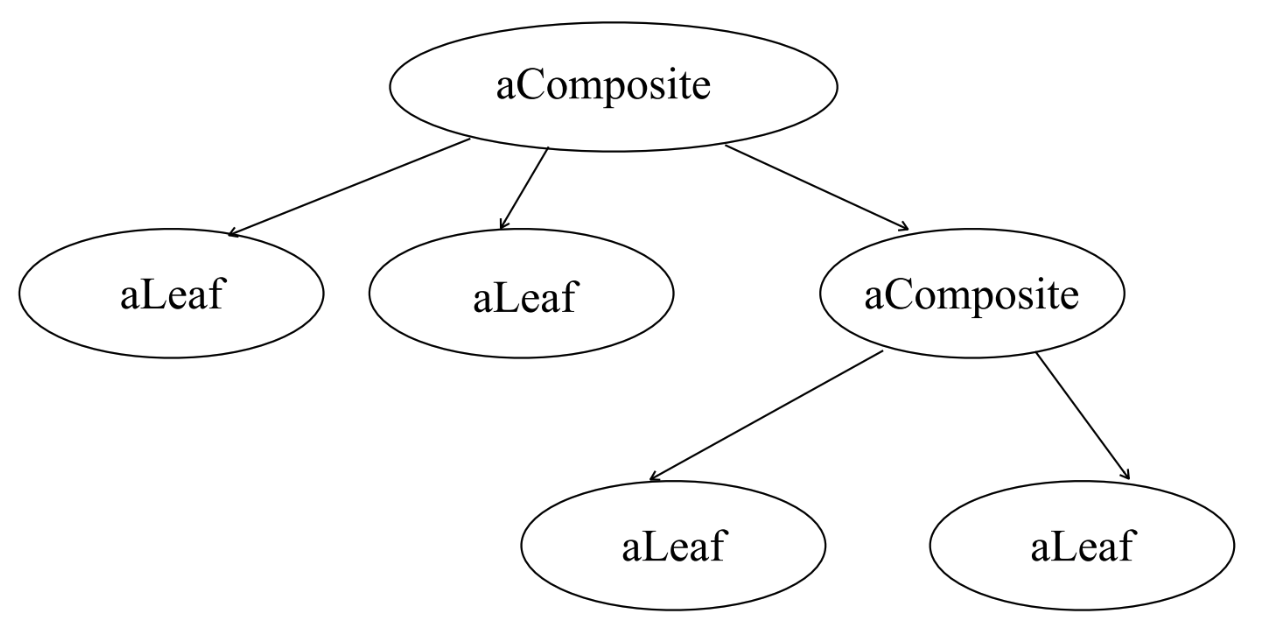
\includegraphics[width=0.6\linewidth]{Pictures/Screenshot 2023-02-05 at 12.30.50.png}
\end{figure}
\subsubsection*{General UML}
Composition of objects: Each component can be a leaf, or a composite of another component - which can be a leaf or a composite. \\
In this UML diagram, Client class doesn't refer to the Leaf and Composite class directly, it refers to the common interface to treat both Leaf and Composite in the same way.
\begin{figure}[H]
    \centering
    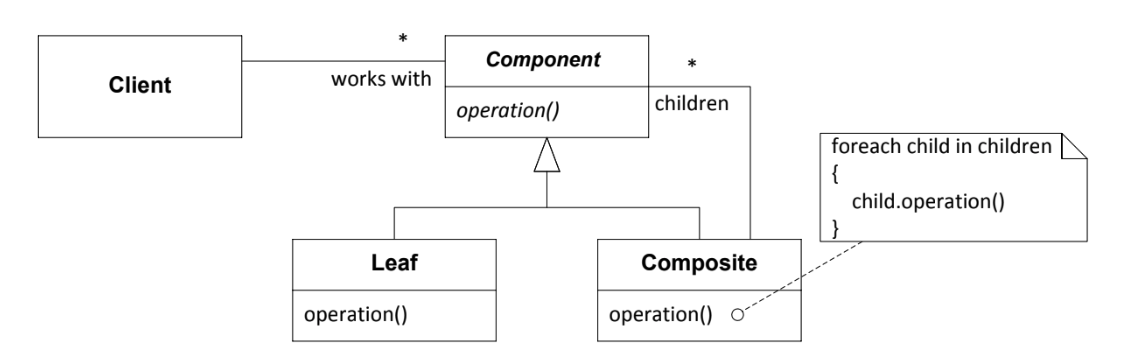
\includegraphics[width=0.8\linewidth]{Pictures/Screenshot 2023-02-05 at 12.32.37.png}
\end{figure}
\subsubsection*{Disadvantages}
Sometimes this pattern is too general, so it is difficult to restrict the objects which can be included in the composite group. \\
Futhermore, since the Composite class has to be extended to provided access to individual group members, then the client code which be able to tell the different between composite objects and non-composite objects.
\subsection{Decorator}
Decorator pattern allows us to add functionality without changing the original class
\subsubsection*{Problem}
We want to introduce a facility into our drawing editor which allows frames to be added to arbitary objects e.g an image
\begin{figure}[H]
    \centering
    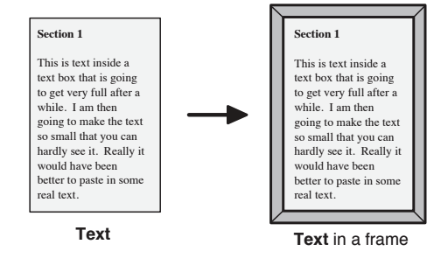
\includegraphics[width=0.5\linewidth]{Pictures/Screenshot 2023-02-05 at 12.35.44.png}
\end{figure}
\subsubsection*{Optimal Solution}
We add a single new subclass of Shape called FramedShape. This has a pointer to a Shape object, which is the shape contained in the frame.
\begin{figure}[H]
    \centering
    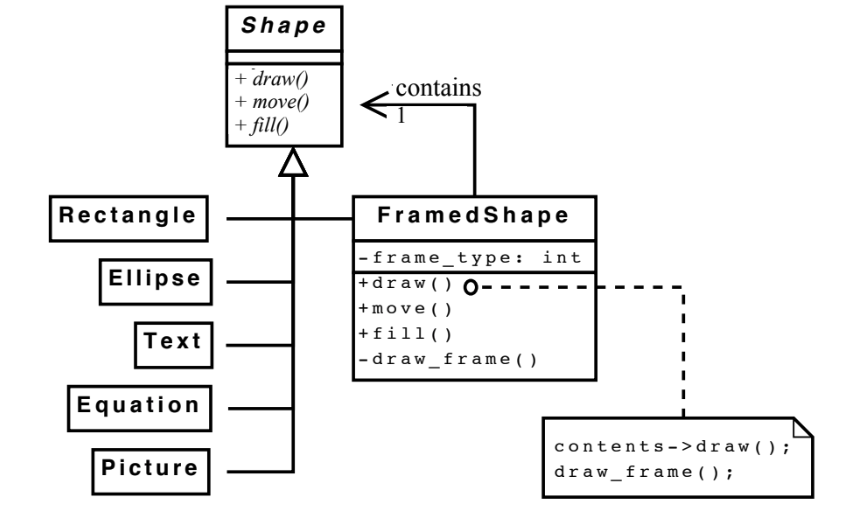
\includegraphics[width=0.6\linewidth]{Pictures/Screenshot 2023-02-05 at 12.36.52.png}
\end{figure}
This means that we can frame any object, and even create a frame around a FramedShape. \\
The object structure would then be like:
\begin{figure}[H]
    \centering
    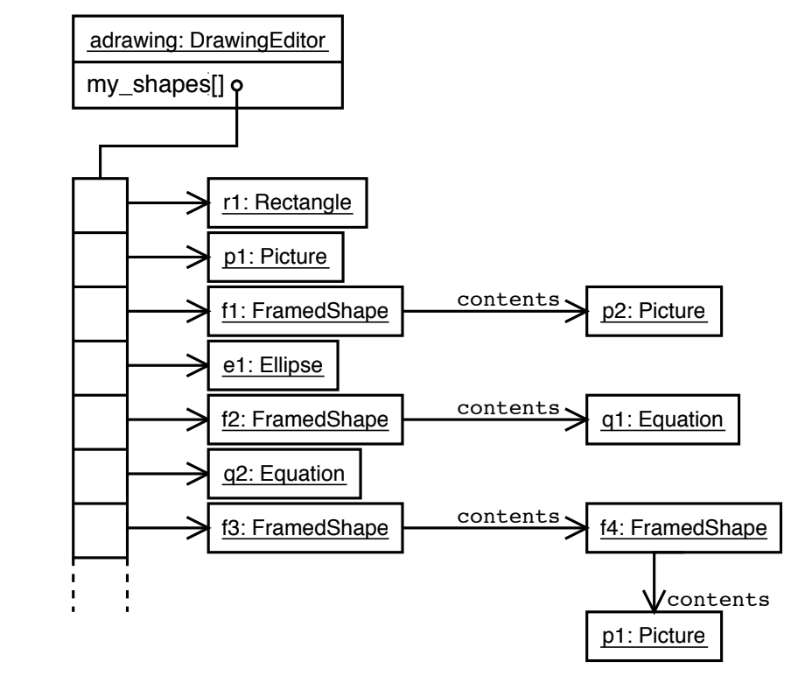
\includegraphics[width=0.5\linewidth]{Pictures/Screenshot 2023-02-05 at 12.38.02.png}
\end{figure}
\subsubsection*{General UML}
This pattern allows us to add optional functionality to all classes, without changing the code for either the base class or any of the subclasses. Multiple decorations can even be added to an object.
\begin{figure}[H]
    \centering
    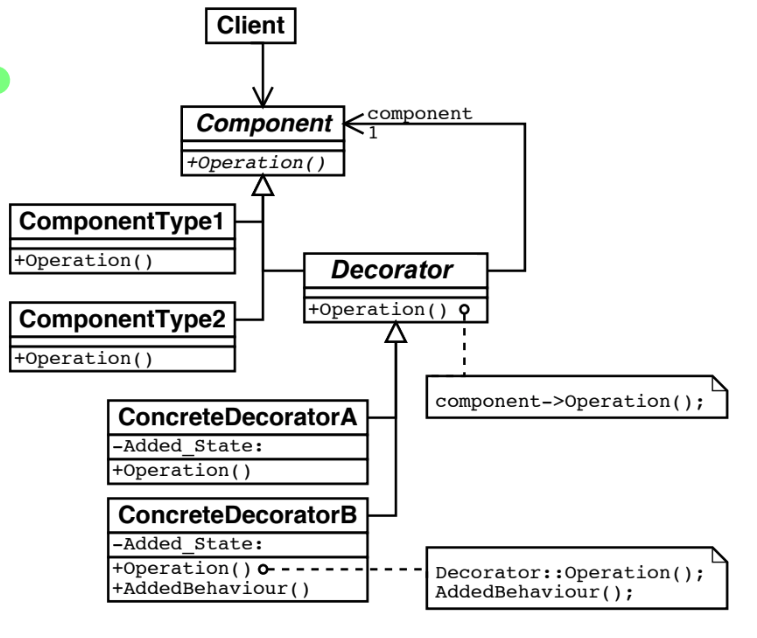
\includegraphics[width=0.6\linewidth]{Pictures/Screenshot 2023-02-05 at 12.39.52.png}
\end{figure}
\subsubsection*{Disadvantages}
If there are not too many kinds of added functionality, and they appear fairly common, then might as well manually add to each class. \\
Also, not even class should become a decorator class. In a running system, can cause a long chain of small objects which all point to each other.
\begin{figure}[H]
    \centering
    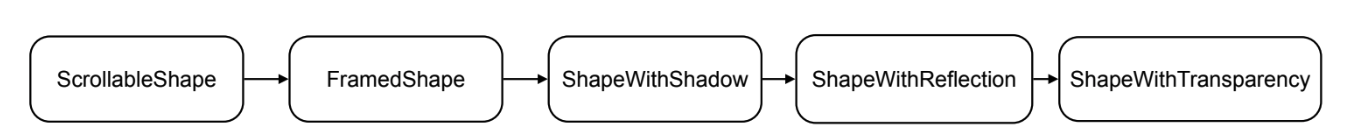
\includegraphics[width=0.7\linewidth]{Pictures/Screenshot 2023-02-05 at 12.42.17.png}
\end{figure}
\subsection{Observer}
For this pattern, an object known as a subject maintains a list of dependents, known as its observers, and notifies them of any changes in its state. \\
\subsubsection*{Problem}
A Business News Publishers needs to inform its News Subscribers who need to be updated as soon as the news comes out.
\begin{figure}[H]
    \centering
    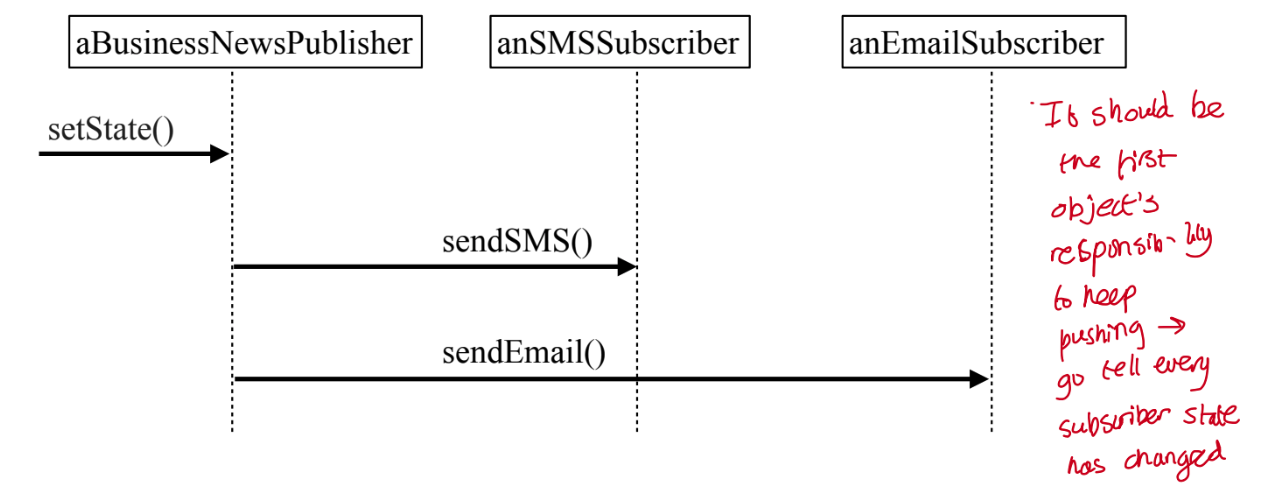
\includegraphics[width=0.6\linewidth]{Pictures/Screenshot 2023-02-05 at 12.46.07.png}
\end{figure}
But we want to extend the system to introduce more different types of subscribers. This pollutes the BusinessNewsPublisher class, and they don't need to know anything about Subscribers. The key relationship here is one to many.
\subsubsection*{Optimal Solution}
NewsProvider doesn't update the state of dependent objects directly, instead Subscriber interface is called by NewsPublisher to update the state.
\begin{figure}[H]
    \centering
    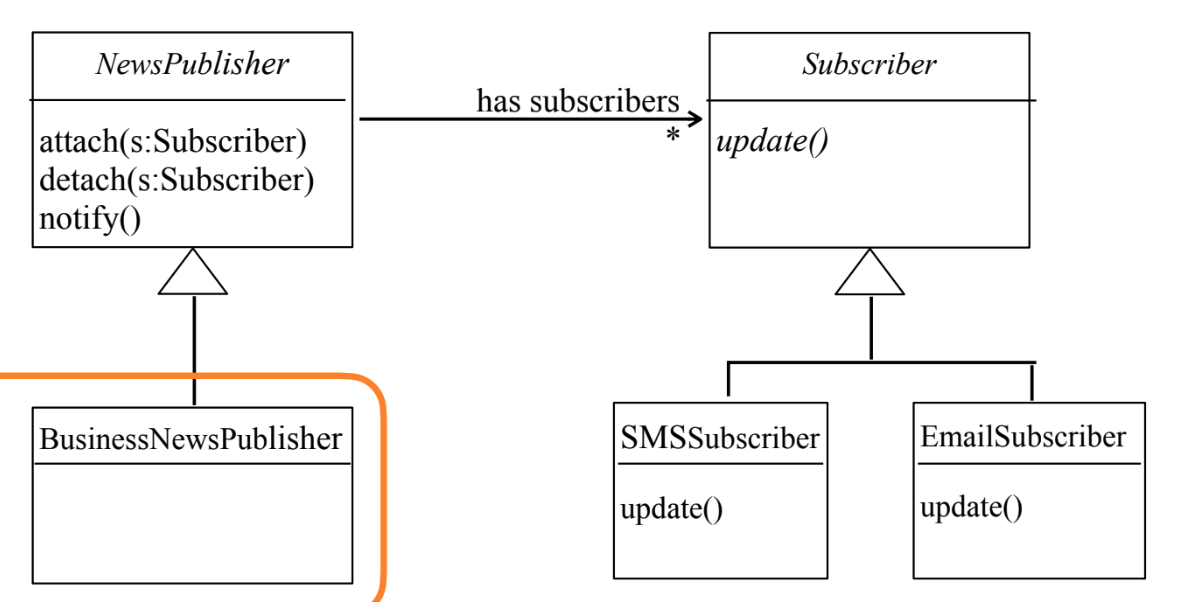
\includegraphics[width=0.6\linewidth]{Pictures/Screenshot 2023-02-05 at 12.48.04.png}
\end{figure}
\subsubsection*{Class Diagram}
This allows multiple objects to maintain a consistent view on the state of the subject.
\begin{figure}[H]
    \centering
    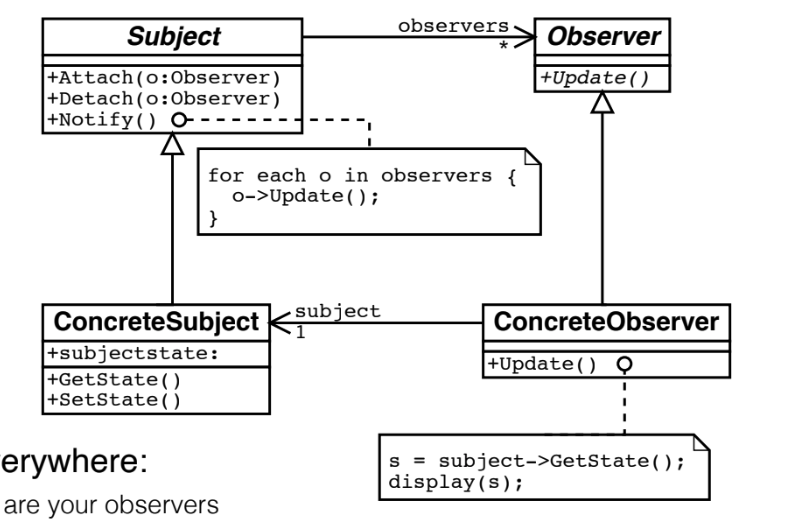
\includegraphics[width=0.6\linewidth]{Pictures/Screenshot 2023-02-05 at 12.49.04.png}
\end{figure}
\subsubsection*{Sequence Diagram}
\begin{figure}[H]
    \centering
    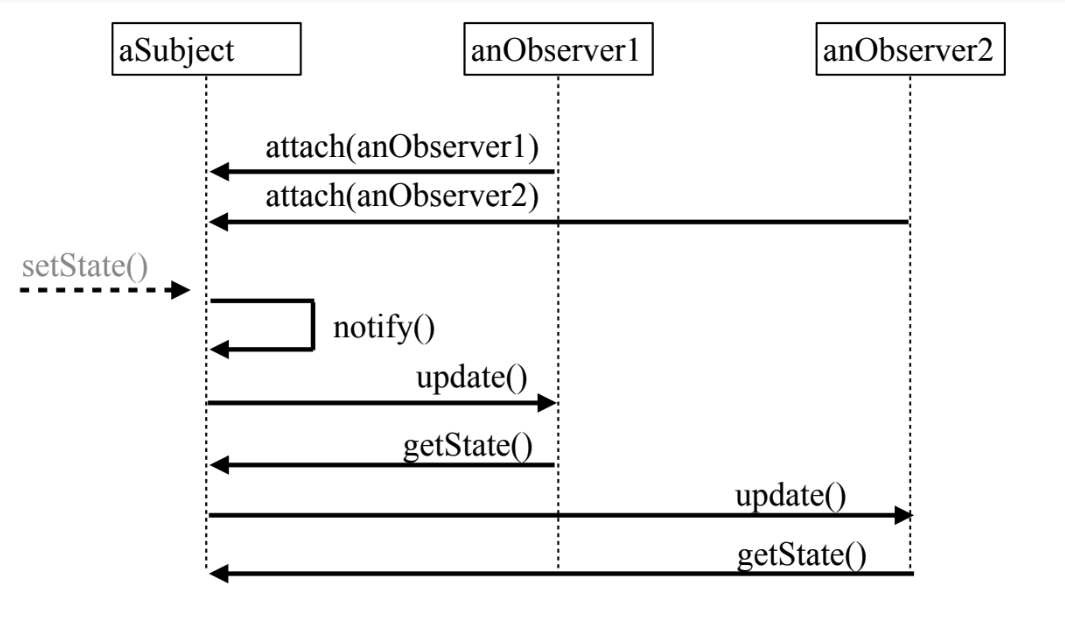
\includegraphics[width=0.6\linewidth]{Pictures/Screenshot 2023-02-05 at 12.49.43.png}
\end{figure}
\subsubsection*{Disadvantages}
This pattern could lead to a large amount of computational overhead if not safe-guarded e.g if the rate of notifications is high, and the reaction to these updates is a heavy-load operation.
\subsection{Model - View - Controller}
These are architectural pattern, which utilise design patterns. \\ The Model-View-Controller (MVC) is the common pattern which seperates the data, its presentation and how it is manipulated by the user.
\begin{figure}[H]
    \centering
    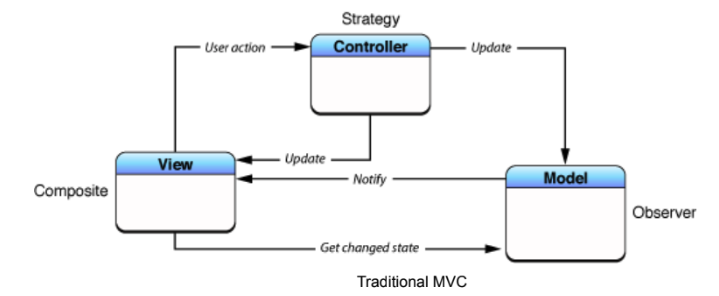
\includegraphics[width=0.6\linewidth]{Pictures/Screenshot 2023-02-05 at 12.52.08.png}
    \caption{Model-View-Controller}
\end{figure}
The individual elements are:
\begin{itemize}
    \item Model - an abstraction of the data that provides ways of accessing and manipulating it
    \item View - presents a specific purpose view onto the Model, captures User's input, then passes it on to the Controller
    \item Controller - interprets User's input and invokes corresponding actions onto the Model
\end{itemize}
\subsubsection*{Passive Mode}
The Controller is the only class that affects the Model. The Controller has to modify the Model based on user's action, then the Controller notifies the View that it has to be updated. The View gets the Data from the Model, and updates itself.
\begin{figure}[H]
    \centering
    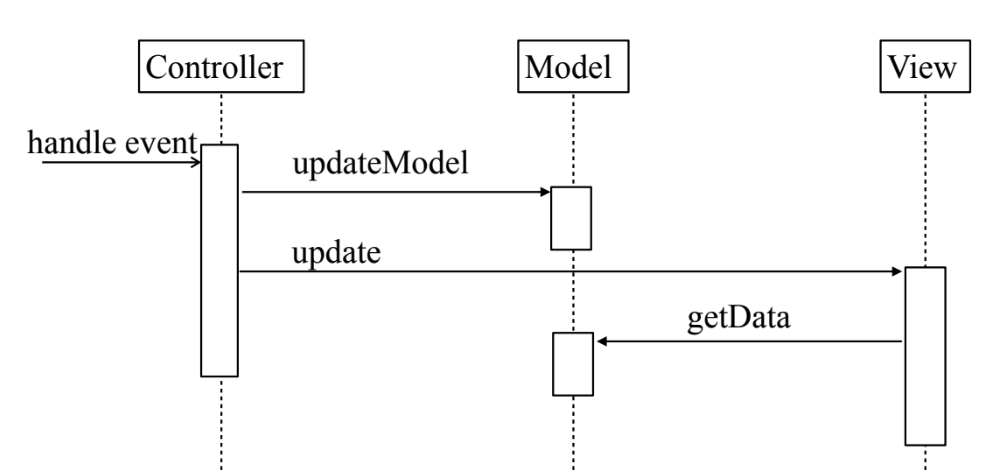
\includegraphics[width=0.6\linewidth]{Pictures/Screenshot 2023-02-05 at 12.55.35.png}
\end{figure}
\subsubsection*{Active Mode}
The Controller is not the only class that affects the Model. After the Model is updated, the Model notifies the View and other classes about updates (Observer Pattern). \\ The View implements the Observer interface, whereas the Model is a subject.
\begin{figure}[H]
    \centering
    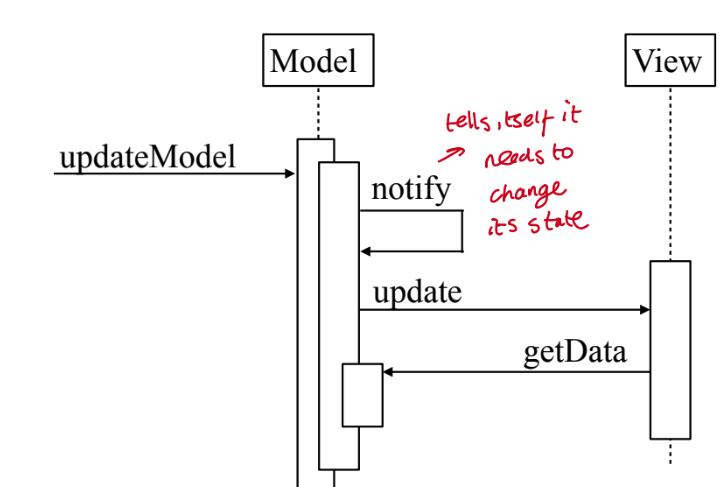
\includegraphics[width=0.6\linewidth]{Pictures/Screenshot 2023-02-05 at 12.57.24.png}
\end{figure}
There is also a variation, where all notifications of state changes in Model to come to the View through the Controller.
\begin{figure}[H]
    \centering
    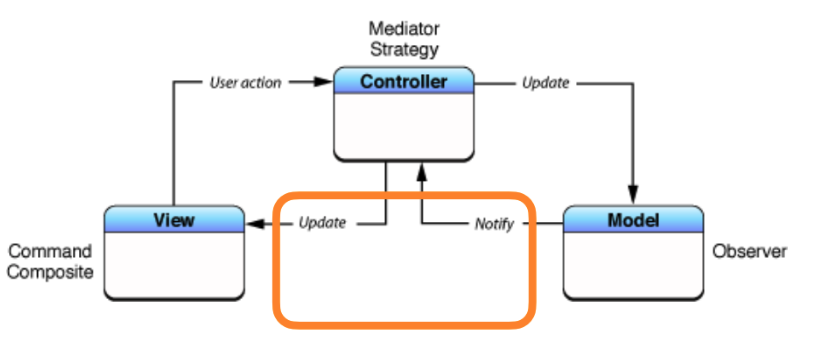
\includegraphics[width=0.6\linewidth]{Pictures/Screenshot 2023-02-05 at 12.58.26.png}
\end{figure}
\subsection{Mobile App Store Design Example}
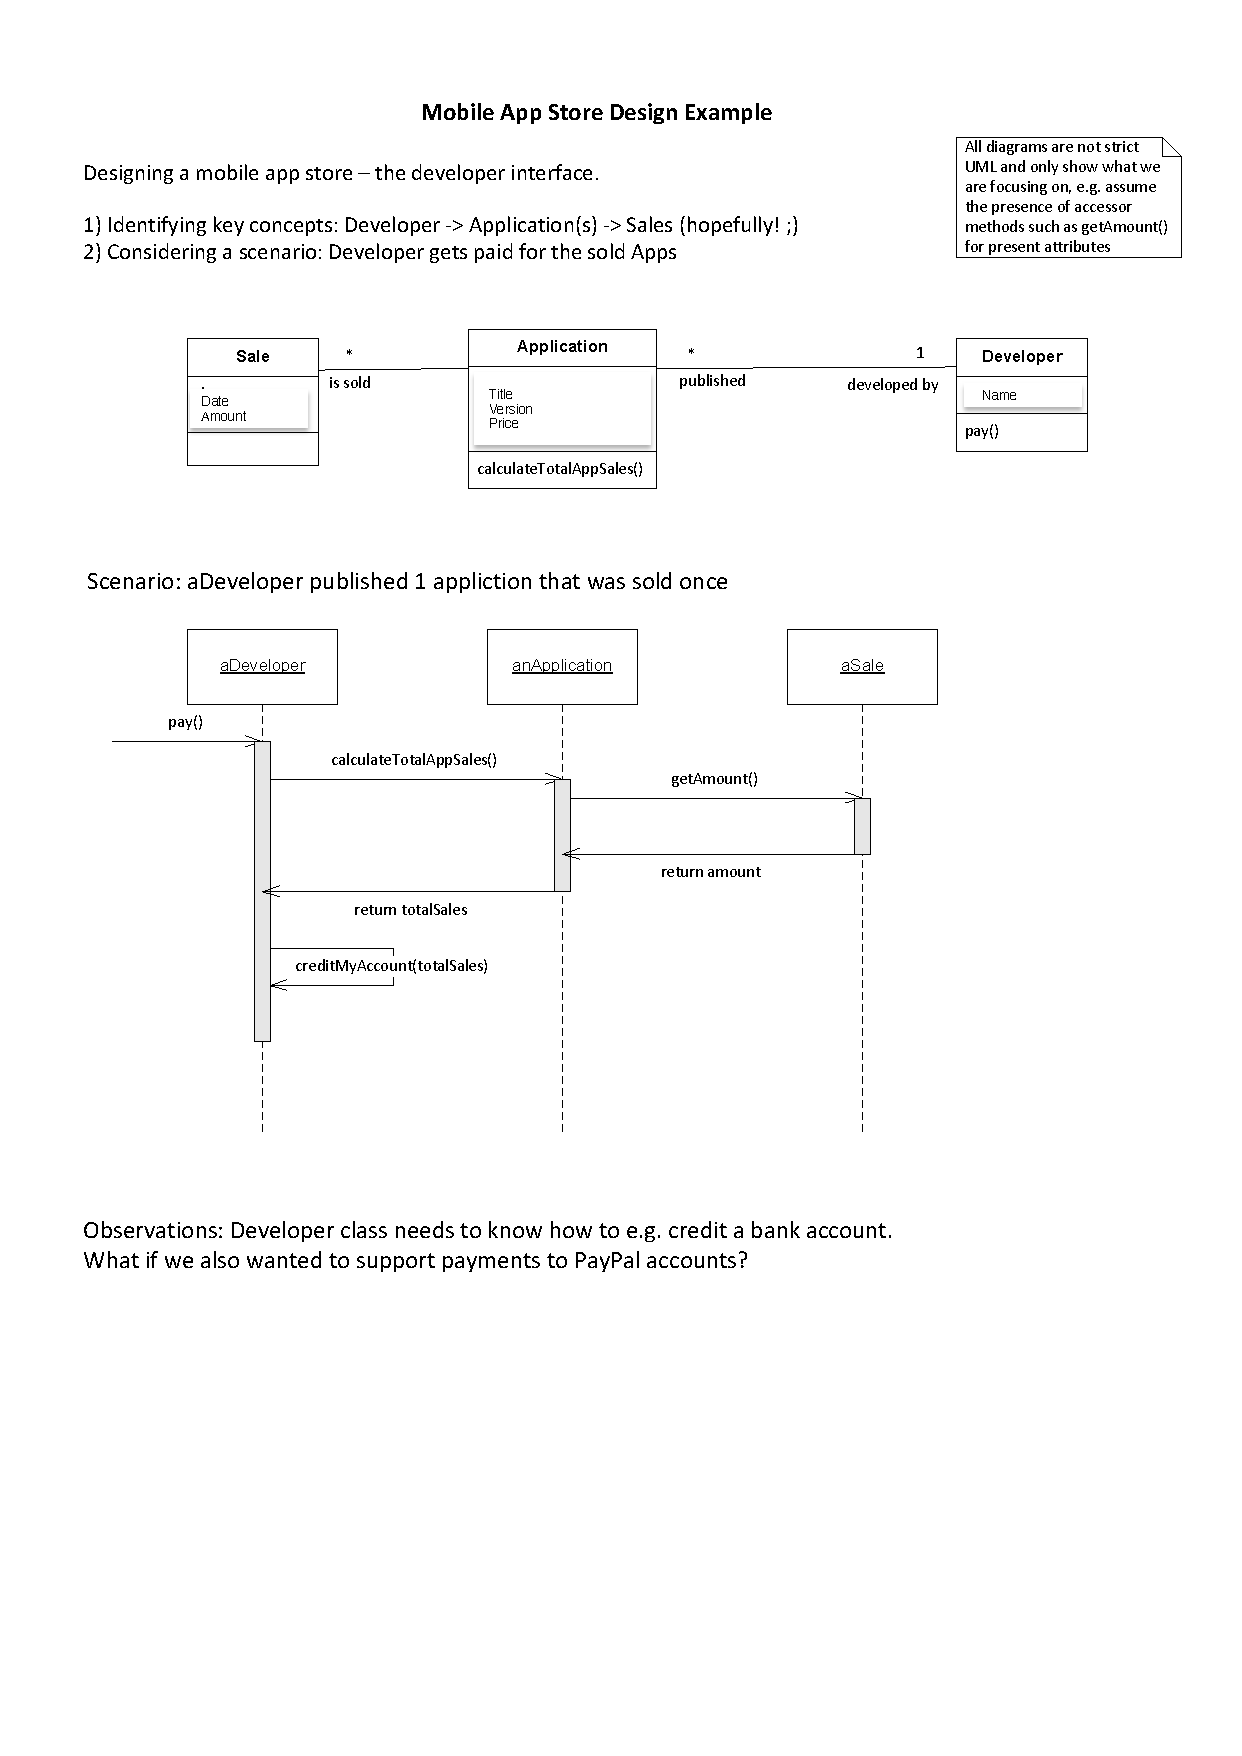
\includepdf[pages=-]{Assets/Mobile_Example.pdf}
What if we now have new requirements? When a sale is made:
\begin{itemize}
    \item The developer should be notified by email
    \item Analytics View showing all sales should be updated
\end{itemize}
\begin{figure}[H]
    \centering
    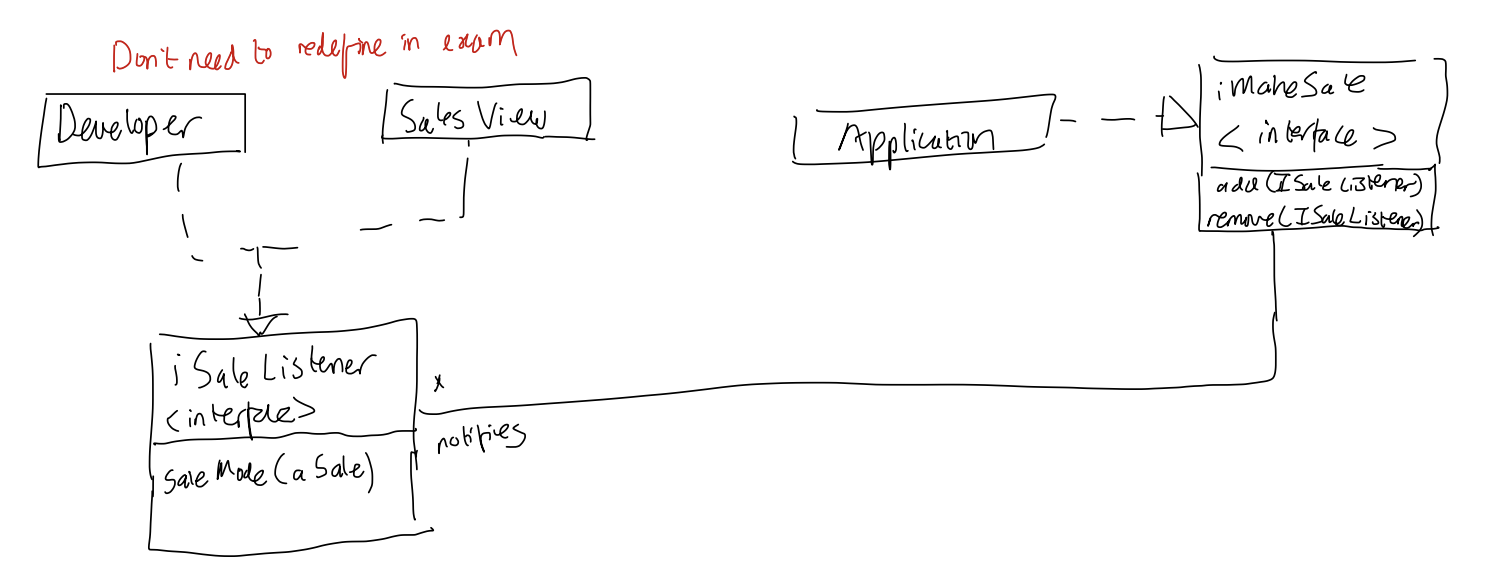
\includegraphics[width=0.8\linewidth]{Pictures/Screenshot 2023-02-08 at 11.55.08.png}
\end{figure}
\begin{figure}[H]
    \centering
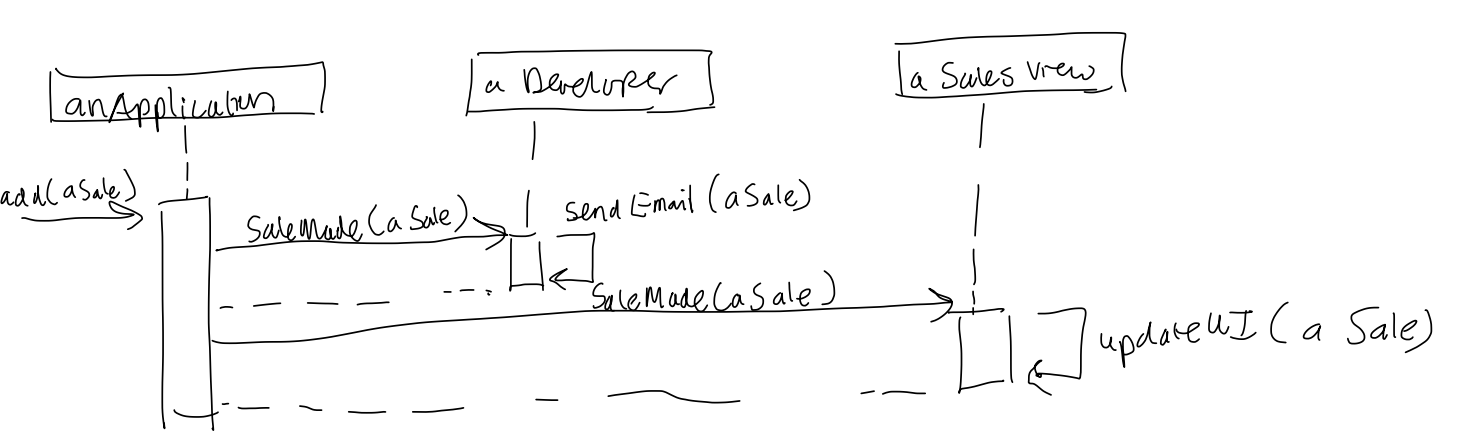
\includegraphics[width=0.8\linewidth]{Pictures/Screenshot 2023-02-08 at 11.55.20.png}
\end{figure}
\section{Lecture 6 - Software Development Methodologies}
\subsection{Waterfall Model}
There is a basic traditional waterfall model for developing software based on the software process \eqref{sp}:
\begin{figure}[H]
    \centering
\includegraphics[width=0.6\linewidth]{Pictures/Screenshot 2023-02-08 at 12.13.38.png}
\end{figure}
The advantages of this model are:
\begin{itemize}
    \item Early clarification of system goals
    \item Can charge for changes to the requirements
    \item Works well with management tools
\end{itemize}
The disadvantages of this model are:
\begin{itemize}
    \item Iterations are critical to software development process, and aren't highlighted in this model
    \item A lot of time is taken on getting the system absolutely right from the beginning
\end{itemize}
\subsection{Traditional Team}
In a traditional team there is:
\begin{itemize}
    \item Architect: principal designer $\rightarrow$ defines the overall architecture, module structure and all major interfaces. Responsible for Specification and High Level Design
    \item Project Manager: scheduling/rescheduling the work, tracking progress and ensuring all process steps are properly completed
    \item Lead programmer: Lead of programming team, will spend 30\% of his/her time managing rest of team
    \item Programmer: Implements specific modules + module test procedures
    \item Tester: Designs test + validation procedures for completed software. These are based on initial specification, and will focus on overall product.
\end{itemize}
Gantt charts can be used to show tasks over the timeline with milestones and dependencies.
\begin{figure}[H]
    \centering
\includegraphics[width=0.8\linewidth]{Pictures/Screenshot 2023-02-08 at 12.17.55.png}
\caption{Gantt Chart}
\end{figure}
\subsection{Spiral Model}
This model allows you to manage risk and handle unknown problems after the project has started. This is done by developing prototypes. Each spiral is a phase, and the radius represents costs so far. The number of spirals depends on the project.
\begin{figure}[H]
    \centering
\includegraphics[width=0.6\linewidth]{Pictures/Screenshot 2023-02-08 at 12.27.15.png}
\caption{Spiral Model}
\end{figure}
The advantages of this is that:
\begin{itemize}
    \item Iterative development with systematic aspects of waterfall model
    \item Iterative incremental refinement through each time around spiral
\end{itemize}
The disadvantages are:
\begin{itemize}
    \item Costly: Expensive to go through the software process everytime
    \item Complexity: hard to understand for new teams to software development
\end{itemize}
\subsection{Evolutionary Model}
These have iterative (with feedback from users) and incremental (consists of smaller incremental waterfall models) delivery
\begin{figure}[H]
    \centering
\includegraphics[width=0.6\linewidth]{Pictures/Screenshot 2023-02-08 at 12.33.18.png}
\caption{Evolutionary Model}
\end{figure}
The advantages are:
\begin{itemize}
    \item Flexible: easy to make changes based on user input
    \item Faster delivery of code
\end{itemize}
The disadvantages are:
\begin{itemize}
    \item If the system deliverables can't be easily split into version which can be delivered to the consumer incrementally, then this model is not ideal
    \item Scope creep: The scope can expand infinitely over time if not careful
    \item Can have a lack of a clear plan if you are just focusing on prototypes
\end{itemize}
\subsection{Testing}
Testing is important as people work in teams. Thus trust is essential, and defects destroy the trust required for effective software development.
\subsubsection{What is Testing?}
Testing is double checking. 
\begin{quote}{Andrew Hunt and David Thomas, The Pragmatic Programmer}
Finding bugs is somewhat like fishing with a net. We use fine, small nets \textbf{(unit tests)}
 to catch the minnows, and big, coarse nets \textbf{(integration tests)} to catch the killer sharks.
\end{quote}
\subsubsection{What to Test?}
We have several different types of tests:
\begin{itemize}
    \item Unit test: code that exercise a small unit of software seperate from other units of application. Foundation of all other types of testing - if the parts don't work by themselves they won't work together
    \item Integration testing: seeing how all the parts interact with each other. With good OO design in place, should be easy to find the issues
    \item Validation and verification: Does the code fit what the user needs, are the functional requirements met?
    \item Resource Exhaustion: check if the system works well in the real-world. Could it run out of memory, disk space, CPU bandwidth etc
    \item If it has to fail, will it fail gracefully
    \item Performance Testing: What if number of users/connections increases. Is it scalable?
    \item Usability Testing: Will it work with real users under real conditions. Also is it intuitively clear how to use
\end{itemize}
Note that tests are also software, need to test them.
\subsubsection{Regression Tests and Test Data}
Regression tests:
\begin{itemize}
    \item Compares the output of previous test with previous/known values
    \item Makes sure that bugs fixed today don't break something else
    \item Use regression tests to make sure that components function correctly, entire subsystem functions, performance etc
\end{itemize}
Test Data:
\begin{itemize}
    \item Real world - typical data collected. We use this as it might reveal misunderstandings
    \item Synthetic - artificially generated data. We use this as we might not have enough real data, or need certain properties to test
\end{itemize}
\subsubsection{How to Plan Testing}
Testing Quadrants:
\begin{figure}[H]
    \centering
    \includegraphics[width = 0.9\linewidth]{Pictures/Screenshot 2023-02-11 at 15.41.28.png}
\end{figure}
This splits tests based on:
\begin{itemize}
    \item Where they are Business-Facing (described to business expert) or Technology-Facing (developer domain)
    \item Where they support software development process, or used to critique the product
\end{itemize}
\textbf{Q1 Technology-Facing/Supporting Development} 
\begin{itemize}
    \item Testing Quadrant: Unit Tests, Component Tests, Deployment Tests
    \item Deployment Tests are performed whenever on deploys the application, to check if it is installed and configured correctly
\end{itemize}
\textbf{Q2 Business-Facing/Supporting Development}
\begin{itemize}
    \item Testing Quadrant: Functional, Prototypes, Simulations, Acceptance
    \item Acceptance Tests: conducted by consumer to verify that system meets the acceptance criteria of application
    \begin{itemize}
        \item Should be written and automated by consumer/users before development starts
        \item Answers the questions: For developers (How do I know when I am done), for users (Did I get what I wanted)
        \item Should run in production
    \end{itemize}
    \item Functional Acceptance Tests: acceptance tests that concern the functionality of the system
\end{itemize}
\textbf{Q3 Business-Facing/Critique the Product}
\begin{itemize}
    \item Testing Quadrant: Exploratory, Usability, User Acceptance, Scenarios, Alpha/Beta
    \item Checking that the specification is correct
    \item Applications are never specified perfectly in advance: always room for improvement, or users try things they are not supposed to
    \item Showcases: show new functionality to the users to catch misunderstandings early
    \item Exploratory: Tester controls the design of tests as they are performed, and uses that to design new and better tests
    \item Beta: Release new features to a select group of real users without them noticing
\end{itemize}
\textbf{Q4 Technology-Facing/Critique the Project} 
\begin{itemize}
    \item Testing Quadrant: Performance, Load, Security
    \item Acceptance Tests can test other qualities of system e.g capacity, usability, security
\end{itemize}
\subsubsection{When to Test}
We should test as soon as we have code, frequent testing reduce costs and defects
\subsubsection{Who Should Test}
We should automate tests as much as possible. Developers hate testing, and it can be very tedious. \\
The goal of automated tests is to reach 100\% coverage, i.e coverage the most practically possible number of test cases. \\
We can use profiling tools to analyse software performance e.g tracking Memory Allocation to spot memory leaks and inefficient memory use.
\subsubsection{Analytics}
Once the product is live with user, we need to get some analytics. \\
This is when we collect and analyse data on product's use to increase product's performance in market. Example metrics would be daily active users, conversion (how many users signed up/made a purchase), engagement.
\section{Lecture 7 - Agile Development}
We do all of this because keeping the system in production has a lot of benefits:
\begin{itemize}
    \item Allows more frequent feedback from colleagues
    \item Release more important features earlier
\end{itemize}
However comes at a cost:
\begin{itemize}
    \item More intense collaboration between departments
    \item More effort to deploy regularly
\end{itemize}
\subsection{Extreme Programming (XP)}
The driving point behind this was: improve software quality, reduce cost of change. \\
XP Values: \textbf{Communcation, Simplicity, Feedback, Courage, Respect} \\
XP Principles:
\begin{itemize}
    \item \textbf{Accepted Responsibility} - responsibility can't be assigned only accepted
    \item \textbf{Economics}
    \item \textbf{Mutual Benefits} - every activity should benefit everyone concerned e.g automated testing
    \item \textbf{Self-similarity} - copy structure of new solution in different context
    \item \textbf{Improvement}
    \item \textbf{Diversity}
    \item \textbf{Reflection}
    \item \textbf{Flow} - deliver steady flow of software
\end{itemize}
Primary XP Practices:
\begin{itemize}
    \item Pair programming
    \item Stories - move from requirements to stories with description of one functionality per story
    \item Weekly cycle and Quarterly Planning
    \item Test-First programming (TDD)
\end{itemize}
\subsection{Continuous Integration (CI)}
Idea behind it: integration is unpredictable, so should integrate and test changes every few hours. Only once the entire test suite has passed should you continue. \\
Key ingredients: Source Repo, Automated Build, Agreement of team. 
\subsubsection{Automated Build} 
Everything should be included, so that someone can be bring in a new machine, check everything out and have a running system on their machine 
\subsubsection{Key Practices} 
\begin{itemize}
    \item Maintain a single main branch
    \item Automate the build
    \item Make your build self-testing
    \item Test in clone of production environment
\end{itemize}
\subsubsection{CI Software} 
Check with your repo if any commits have occurred. If so check out latest version of software, run build script, run tests to notify results. Examples include TravisCI.
\subsection{Continuous Delivery (CD)}
We want to build software that is always in a production ready state. This is done by running a deployment pipeline that tests whether the deployment is in a state to be delivered.
\subsubsection{Deployment Pipeline}
This is an automated software delivery system. The stages are:
\begin{enumerate}
    \item Developers commit changes in their source repo. The first commit complies the code, runs the tests, if all ok then turn the executable code into binaries and store in binary repo.
    \item Longer running automated acceptance tests
    \item Pipeline branches to enable independent deployment of your builds in various environments. Testers should be able to see release candidates available, and deploy in relevant environments. 
\end{enumerate}
\begin{figure}[H]
    \centering
    \includegraphics[width = 0.8\linewidth]{Pictures/Screenshot 2023-02-11 at 16.30.40.png}
    \caption{CD Pipeline}
\end{figure}
\section{Lecture 8 - Software Entrepreneurship}
\subsection{Innovation}
Innovation is about converting research into products. They provide software systems which change the practices of their user communities. But the more real innovation you have, the longer it takes to bring it to market. \\
Timing also matters, is the market ready for your innovation? What is required to bring the innovation to the market? \\
An innovative product must:
\begin{itemize}
    \item Display novelty: hasn't been developed before
    \item Display utility: has some form of application that users value and are prepared to pay for
\end{itemize}
Start-ups are great for getting to new markets as they:
\begin{itemize}
    \item Have a team of dedicated and focused people
    \item Have nothing to lose
    \item No targets to meet
    \item No established business models to protect
\end{itemize}
When defining an start-up idea, need to understand:
\begin{itemize}
    \item Is it a product or a service: affects how much you charge for it, how much resources you need to grow
    \item Is there an established market for this product, or is there a new market to create
    \item If there is an established market, is it growing or saturated
    \item Has someone else done it, how successful are they, what can be learnt from them
    \item How big is the total market
    \item How could the market be accessed
\end{itemize}
\subsection{Market Research - Gartner Curve (Hype Cycle)}
We can use this curve to analyse trends.
\begin{figure}[H]
    \centering
\includegraphics[width=0.6\linewidth]{Pictures/Screenshot 2023-02-15 at 14.18.38.png}
\end{figure}
\subsection{Markets}
We also need to understand the competitors, size, sales etc. Also if the market trends are growing/consolidating. \\
There are several market types:
\begin{itemize}
    \item New product/existing market: improving a well-defined value proposition e.g LED bulb
    \item New product/an existing market and re-segmenting as a low-cost proposition: improving value-for money ratio e.g low-priced Android phone
    \item New product/existing market and re-segmenting as a niche proposition: focusing on a segment of the market e.g speciality coffee
    \item New product/new market: customers don't know they need it e.g instant messaging
    \item Implementing a proven successful value proposition in a new country: can adapt to cultural differences e.g XING, Linkedin in Germany
\end{itemize}
\subsection{Business Plan}
We have this so that internally: can convince teammates and yourself, and externally: to raise funds. \\ It normally consists of a part showing how it will be developed into a profitable company. Rarely asked for today. \\
Also need to think about product/market fit:
\begin{itemize}
    \item Who are the customers who need the product
    \item Does the product solve the problem
    \item Are these customers prepared to pay the price for the value they are getting
    \item Is this business going to be sustainable if selling the product to customers at this price
\end{itemize}
\section{Lecture 9 - Human-Computer Interaction Introduction}
Human-Computer Interaction (HCI) requires a system approach. Thus, we need to consider the full socio-technical context when design these systems. Even if we focus on a subsystem, successful deployment relies on the ability to understand and relate observations, to their wider, system-level context. \\ The purpose of HCI is to impact the design of applications, interaction techniques, systems or services so users can achieve their goals in an effective, efficient, safe and satisfactory manner. \\
Note, there is no perfect design - it is all about identifying tradeoffs, and creating new ideas. \subsection{Types of Research in HCL}
\subsubsection*{Empirical Problems}
These are where we find phenomena in interaction based on empirical data. For example, seeing the consequences of social media on relationships. 
\subsubsection*{Conceptual Problems}
Explaining previously unconnected phenomena occurring in interaction using theory. For example, building a theory of what it means for users to be immersed in VR
\subsubsection*{Constructive Problems}
These are mostly about how we build systems. For this, we tackle the knowledge needed for constructing interactive systems for some stated purpose in human use of computing.
\subsection{HCI Practitioners}
HCI Practitioners work to create an understanding of their users and their activities. They also evaluate interactive systems from the users perspective e.g testing the systems with users. 
\subsection{Fundamental Concepts}
\begin{figure}[H]
    \centering
    \includegraphics[width=0.8\linewidth]{Pictures/Screenshot 2023-02-17 at 12.17.25.png}
\end{figure}
\subsubsection{Human-Centred}
HCI is human-centred $\rightarrow$ focuses on the people who use an interactive system, or who are affected by this use. This means that they need to:
\begin{enumerate}
    \item Understand users
    \item Engage with people
    \item Have an ethical consideration of how an interactive system may directly/indirectly affect people
\end{enumerate}
Systems should match people, rather than the other way around. We want to have the best possible understanding of people. \\
The primary rationale for any practical decision should be rooted on understanding of the people using or affected by the system. An example is:
\begin{figure}[H]
    \centering
    \includegraphics[width=0.7\linewidth]{Pictures/Screenshot 2023-02-17 at 12.21.24.png}
\end{figure}
\subsubsection{Interaction}
This refers to the reciprocal influence between people, and an interactive system that takes place through the user interface. This is complex, as it not singularly defined by the user nor the computer. Thus, it often involves co-adaption between people and computers.
\subsubsection{User Interfaces}
A user interface is the parts of an interactive system that the user comes into contact with.
\subsubsection{Design}
Designing - the process of arriving at a plan, specification, prototype, system. This can involve a user interface, and relevant parts of the underlying interactive system, but also a service.
\subsubsection{Engineering}
This is using technical principles e.g maths and science, to realise a design that best meets a given set of expectations.
\subsubsection{Evaluation}
This refers to an application of some systematic methodology to attribute some human-related value to an artifact, prototype, system or process. There are 3 main variants of evaluation:
\begin{itemize}
    \item Verification - ensuring that the design meets all requirements and constraints for the design task
    \item Validation - ensuring that the design is fit for its intended purpose
    \item Testing - refers to carrying out evaluation by means of trying something out in realistic conditions
\end{itemize}
\subsection{Why HCI Matters}
Humans have an egocentric fallacy - we assume that others are like us, and thus can design systems which are not simple for everyone to understand. Thus, we need to make interactive systems easier. It is also more profitable, as it can lead to:
\begin{itemize}
    \item Market pull - sensing there is market demand for a new offering
    \item Technology push - new technology is injected into the market, and thus generates new demand for something which was previously unavailable.
\end{itemize}
\subsection{Approach}
We focus on principles and skills. By principle, we mean a foundational idea that explains how some happens in human-computer interaction. For example, \textbf{Direct Manipulation} states that computational objects must be presented on a display and acted on by the user through direct, reversible and incremental actions with immediate feedback.
\section{Understanding People}
There are several types of understanding, these include:
\begin{enumerate}
    \item Theories: consist of constructs and relations amongst those constructs
    \item Concepts: name particular phenomena, how to identify the phenomena, where they usually occur, and their underpinning mechanisms
    \item Taxonomies: system of elements or mechanism of how people feel, think or act
    \item Models: simplifications of reality
    \item Guidelines: theoretical knowledge that can be summarised in practical rules of thumb/heuristics
\end{enumerate}
Note, we can't create user experience, we can only create an interface to allow users to feel something. \\
\begin{center}
\begin{tabulary}{0.99\textwidth}{|p{2.5cm}|C|C|}
    \hline
\thead{Area} & \thead{Focus} & \thead{Relevance for design} \\ 
                    \hline
Perception & How people sense things & Informs the design of user interfaces  \\    \hline
Motor control & How people move & Informs the design of input devices, interaction techniques \\ \hline
Cognition & How people remember, pay attention, think & Informs the design of tasks which require memory and reasoning \\ \hline
Needs & How needs work to motivate people & Tells us what's important for users in computer use \\ \hline
Experience & How people experience/form experiences & Tells us how users experience events involving computers \\ \hline
Communication & How people communicate with each other & Informs design for human-human communication \\ \hline
Collaboration & How people achieve joint goals & Informs design of collaborative software \\ \hline
    \end{tabulary}
\end{center}
We also need to apply our understanding of people:
\begin{itemize}
    \item Direct what to pay attention to 
    \item Explain empirical findings
    \item Make design decisions
    \item Explore a design space
    \item Predict people's behaviour
\end{itemize}
\subsection{Perception}
Perceptions serves a lot of roles in human-computer interaction. We regulate our actions in interaction via perception, and user interfaces communicate their state via perception. \\
There are 3 main processes which contribute to perception:
\begin{figure}[H]
    \centering
    \includegraphics[width=0.3\linewidth]{Pictures/Screenshot 2023-02-22 at 15.33.15.png}
\end{figure}
Although it seems like our experience of the world is veridically (truthfully) reflecting the sensory information we receive, our perception is affected by our expectations which are drawn from prior experiences, along with how we deploy attention to sample attention. \\
We also have sensation - a physiological process that produces information about the environment for perception. This is about transduction - generating output data from input data. \\
Some examples of human sensory modalities ( how human perceive the world using their senses) in HCL are:

\begin{center}
\begin{tabulary}{0.99\textwidth}{|p{3cm}|C|C|}
    \hline
\thead{Sensory Modality} & \thead{Key Characteristics} & \thead{Design considerations} \\ 
                    \hline
    Vision & Fast, field of view about 180º & Visual graphical displays e.g contrast \\ \hline
    Hearing & Very Fast, but can only process information one at a time, 360º field & Properties of sound and voice e.g pitch, melody \\ \hline
    Tactition & Fast, but only areas of physical contact & Properties of haptic simulation e.g amplitude, frequency of vibration \\ \hline
    \end{tabulary}
\end{center}
Some relevant properties we can use are:
\begin{itemize}
    \item Information rate: how much information can be sensed per unit of time
    \item Parallelism: how much parallel processing of information can occur 
    \item Sensitivity: minimum intensity of physical stimulation for receptor to exceed its sensation threshold
    \item Receptive field: Region of space that activates neurons in visual space
    \item Adaption: Tuning of outputs to attenuate non-informative signals
\end{itemize}
Example of some perceptual tasks are:
\begin{itemize}
    \item Discrimination: telling whether a difference occurs in sensory stimulation
    \item Detection: telling whether an event of interest occurs in the environment
    \item Recognition: categorising a stimulus as something
    \item Estimation: estimating a property of an object in the environment
    \item Search: localising an object of interest
\end{itemize}
There are also windows of visibility - we use them to understand how viewing conditions affect perceptual tasks. Some examples are:
\begin{itemize}
    \item Visible spectrum of light - can only perceive in limited range of spectrum of light
    \item Field of view - field of view is limited to 190º horizontally, 125º vertically 
    \item Contrast - difference in color that makes something in field of view stand out
    \item Foveated vision - retinal image is limited, non-uniform. At the periphery it loses accuracy
\end{itemize}
There is also perceptual organisation:
\begin{enumerate}
    \item The division of elements in figure and ground. Some objects belong to a figure, and some belong to the background. We can use this to show a display hierarchy
    \item Their grouping into coherent regions
\end{enumerate}
\subsubsection*{Gestalt Laws}
These are visual grouping rules:
\begin{itemize}
    \item Proximity: group based on how close elements are to each other
    \item Common area: have defined regions, group elements depending on how they fit in these regions
    \item Similarity: elements with similar qualities grouped together
    \item Continuation: elements are connected by continuation of flow
\end{itemize}
\begin{figure}[H]
    \centering
    \includegraphics[width=0.8\linewidth]{Pictures/Screenshot 2023-02-22 at 15.59.34.png}
\end{figure}
\subsubsection*{Visual Saliency}
This is the probability with which visual features attract attention when we see a user interface for this first time. This can depend on the distribution of visual features, expectation (prior experiences on similar designs)
\begin{figure}[H]
    \centering
    \includegraphics[width=0.5\linewidth]{Pictures/Screenshot 2023-02-22 at 16.03.33.png}
\end{figure}
We can also use ths to explain how cluttered a display is perceived to be, as clutter means that everything on the display attempts to be salient. Imagine trying to play a note on a display. If a display is cluttered, then there is no visual feature which would make the note stand out.
\begin{figure}[H]
    \centering
    \includegraphics[width=0.5\linewidth]{Pictures/Screenshot 2023-02-22 at 16.05.03.png}
\end{figure}
\subsection{Motor Control}
We can personalise graphical layouts to better match a user's motor abilities. This can also be done by making objects on display easier to select. Some elements of a HCI motor task include:
\begin{itemize}
    \item End-effector: the body part we are using to select
    \item Degrees-of-freedom: how many ways we can translate that end-effector in 3D space
    \item Aimed movement: Attempt to move end-effector to certain location
    \item Interception Task: A task with both spatial and temporal demands e.g trying to catch a falling object
    \item Speed-accuracy tradeoff: Higher speed results in lower accuracy
\end{itemize}
\subsubsection*{Fitt's Law}
Fitt's Law models the \textbf{movement time} (MT) it takes for a user to acquire a target with \textbf{index of difficulty} (ID):
\[
MT = a + bID, \; ID = \log_2(\frac{D}{W}+1)
\]
Where D,W are the distance and width to the target, and a/b are regression coefficients. \\
We can use this law to compute input devices using throughput. Throughput is the number of bits a user can communicate independently of a specific target. One way to measure it is:
\[
TP = \frac{ID_{\text{avg}}}{MT_{\text{avg}}}
\]
But this relies on an arbitrary ID. So we can also use:
\[
TP = \frac{1}{b}
\]
This has a downside that it ignores intercept a, but it more commonly used.
\subsubsection*{Crossing}
A crossing task is a target acquisition task that relaxes the stopping constraint of a pointing task (D parameter). This allows the user to select multiple targets in one motion.
\begin{figure}[H]
    \centering
    \includegraphics[width=0.7\linewidth]{Pictures/Screenshot 2023-02-22 at 16.22.52.png}
    \caption{Cluttered display}
\end{figure}
\subsection{Steering}
Steering is when we move a cursor within a tunnel constraint. We can model the time (T) taken for a user to steer a cursor through a tunnel by:
\[
T = a + b \int_C \frac{ds}{W(s)}
\]
Where a,b are parameters, C is the tunnel parameterised by s, and W(s) is the width of the tunnel at s. If we differentiate both sides, with respect to s then we get:
\[
\frac{ds}{dT} = \frac{W(s)}{b}
\]
Thus, instanteous movement speed is proportional to the width of the tunnel. We can also define the index of difficulty for a parameterised curve C as:
\[
ID_C = \int_C \frac{ds}{W(s)}
\]
\begin{figure}[H]
    \centering
    \includegraphics[width=0.5\linewidth]{Pictures/Screenshot 2023-02-22 at 18.21.16.png}
    \caption{Steering}
\end{figure}
A steering task with constraints on both ends, follows the same log relationship as Fitt's Law
\begin{figure}[H]
    \centering
    \includegraphics[width=0.3\linewidth]{Pictures/Screenshot 2023-02-22 at 18.23.08.png}
\end{figure}
\subsubsection*{Simple Reaction}
A simple reaction is when something appears on the display, and the user must respond to it as quickly as possible. We can model this by:
\[
RT = T_d + T_{er} = T_d + x +y
\]
Where RT is the reaction time, $T_d$ is the decision time, $T_{er}$ is the non-decision time, x is the time duration for perceptually encoding the stimulus, and y is the time duration for the motor response.
\subsubsection*{Choice Reaction}
This is when there are n options available. When a cue appears, the user must response as quickly as possible by pressing the correct key. This is open-loop. We can model the decision time as:
\[
\begin{aligned}
T &= bH \\
H &= \sum_{i=1}^n p_i \log_2(\frac{1}{p_i}+1)
\end{aligned}
\]
Where T is the time taken, b is a parameter, and $p_i$ is the probability of each ith choice.
\subsubsection*{Hick-Hyman's Law: Choice Reaction}
This Law comes from if all the choices in a reaction task are equally probable. The average choice reaction time T for n choices is then:
\[
T = a + b\log_2(n)
\]
If there is uncertainty i.e chance of no response, then the formula is:
\[
T= a + b\log_2(n+1)
\]
As no response is just another choice
\subsection{Cognition}
\begin{figure}[H]
    \centering
    \includegraphics[width=0.7\linewidth]{Pictures/Screenshot 2023-02-22 at 18.30.45.png}
\end{figure}
Cognition for HCI relies on:
\begin{itemize}
    \item Supervisory control: adaptively deciding goals, changing course of action when required
    \item Memory: forming, maintaining and accessing beliefs about objects that are not directly perceivable
    \item Attention: selectively processing some part of the perceptual field
    \item Reasoning: applying transformation rules to beliefs to form new beliefs
    \item Decision-making: Interaction can often require making decisions
\end{itemize}
In HCI, the goal often relates to something that people would like the computer to do. This affects how cognition processes information. Human memory is more about offering access to memories that may be useful for a given task. \\
This requires mental effort:
\begin{enumerate}
    \item Task effort: responses to increase computational demands e.g using a new interface
    \item State effort: Energy required to protect performance from physiological fatigue e.g sleep deprivation
\end{enumerate}
\subsection{Needs and Motivations}
There are psychological needs which interactive systems can satisfy:
\begin{center}
\begin{tabulary}{0.99\textwidth}{|C|C|}
    \hline
\thead{Psychological Need} & \thead{Explanation} \\ 
                    \hline
    Relatedness & Need for social relationships \\ \hline
    Meaning & Need for purpose and direction \\ \hline
    Stimulation & Need for novel sensations and thoughts \\ \hline
    Competence & Need for the ability to perform well in important activities \\ \hline
    Popularity & Need for recognition by others \\ \hline
    Security & Need for protection of self from  harm \\ \hline
    \end{tabulary}
\end{center}
\subsection{Collaboration}
Collaboration is a mutual beneficial relationship between 2 or more parties, whereas cooperation means that a division of labor is in place. There is a 2-axis model of collaborative tech:
\begin{figure}[H]
    \centering
    \includegraphics[width=0.7\linewidth]{Pictures/Screenshot 2023-02-22 at 18.40.11.png}
\end{figure}
We also need to consider:
\begin{itemize}
    \item Scale
    \item Nascene: degree of coordination actions that are under development by participants i.e how much freedom do they have to make modifications
    \item Planned permanence: intended stability of collab arrangement
    \item Turnover: stability of a group of participants
\end{itemize}
\section{Lecture 11 - User Research}
Many products fail as their designs fail to realise an understanding of user's needs,wants and motivations. This is why we have \textbf{user research} - principles and methods of empirical research used for obtaining, analysing and representing such knowledge. \\
We do this, as most of the time, the person creating the code is not the user. When we collect data, it should be about actual users engaged in specific activities with specific needs/capabilities. \\ This all forms a key part of \textbf{user-centered design} - understand first and design later. 
\subsection{Obtaining knowledge about users}
\subsubsection{Say-Do problem}
A key problem with users is the \textbf{say/do problem}: what users say they do might differ from what they actually do. This could be because many factors that drive our behaviour are subconscious, or hard to describe verbally. We also have \textbf{tacit knowledge}: knowledge which we are largely unaware of, but can use in the right situation e.g riding a bike. \\
People can also lie for social reasons: i.e exaggerating information to get a positive impression.
\subsubsection{Other reasons}
Other reasons why obtaining knowledge about users is complicated is because users needs might only be recognised in the future. Also, social reasons make it difficult to gain insights into users, as well as the large diversity of users. There might be non-user stakeholders i.e groups which are affected by the system, but don't actual use it.
\subsection{Goals of User Research}
\begin{itemize}
    \item People: user skills, personalities, abilities
    \item Activities: tasks that users do and the practices they engage in
    \item Contexts of use: physical context (lighting), social context (relationships), cultural context (cultural beliefs)
    \item Technologies: existing technologies
\end{itemize}
\subsection{Who is the user?}
To find the user, we need to:
\begin{itemize}
    \item Find a target audience
    \item Sample a set of profiles which accurately describe the target audience
    \item Find stakeholders - these might be people who are affected by the system, indirectly involved in their use, or benefit from the system.
\end{itemize}
\subsection{User Research Methods}
Some examples of user research methods include:
\begin{itemize}
    \item Open-ended interviews: ask users questions about their experiences
    \item Observation: Observe users while trying to avoid affecting them
    \item Diaries: have users keep a diary about their usage
\end{itemize}
\subsection{Research Strategy}
Research strategy is about to how to research methods for gathering insights about users. These are based on several principles:
\begin{enumerate}
    \item There is no correct method, depends on the goal of the research
    \item There are trade offs
    \begin{itemize}
        \item Realism: how similar the situation is to actual thing
        \item Precision: how much accuracy and detail the data is
        \item Generalisability: how well the findings generalise
    \end{itemize}
\end{enumerate}
\subsection{Methodological Quality}
We have to consider \textbf{validity}: whether the conclusions from the study are warranted.\\  We also have to consider \textbf{reliability}: concerns that the user research results in consistent results. \\
Another consideration is \textbf{transparency}: all results and design should be accessible.\\
Finally, we should consider \textbf{ethics}: we have to consider what's right and wrong in collecting and reporting data.
\subsection{Does user research work?}
There are arguments against user research:
\begin{itemize}
    \item Feature creep: adhering to the weakest signal in user research
    \item Users adapt to the systems, even if the systems are not well adapted to human abilities
\end{itemize}
Thus, we should think of user research about informing good designs rather than driving radical innovations.
\subsection{Interviews}
We want to interview, to learn about the subjective experience of users. \\
These can be \textbf{structured}, i.e a fixed set of questions, \textbf{unstructured}, no fixed schedule, or \textbf{semi-structured}, where there is a loose set of questions. These can also be called open-ended interviews.
\subsection{Field Research}
Field research: collection of data on users in their real context. We can do these through observations. But we also need to consider:
\begin{itemize}
    \item Site of observations: where to observe users
    \item Shadowing: follow particular people
    \item Data capture: records of observations for later analysis and verification.
\end{itemize}
\subsection{Survey Research}
This is when a researcher designs a questionnaire, and then distributes it to respondents who fill it in. We can use this to understand users' behaviours, experiences, needs and attitudes. One benefit of survey research is generalizability. 
\subsection{Unobstructive Research}
This is a form of non-interventional user reseach i.e we use traces of users' behaviours to make inference of users and their activities. Some examples of data is:
\begin{itemize}
    \item Direct traces: recording by user's actions
    \item Indirect traces: Only caused indirectly by users e.g walking through a park creating a path
    \item Archive data: social media
\end{itemize}
\subsection{Representations of User Research}
We want to use user research to inform design decisions. That means we have to consider how we represent research data. \\
For example, can use a rich picture to represent the insights from user research in a diagram
\begin{figure}
    \centering
    \includegraphics[width=0.5\linewidth]{Pictures/Screenshot 2023-02-26 at 18.55.31.png}
    \caption{Rich Picture about a pub}
\end{figure}
\subsection{Requirements}
We use user requirements in software engineering to specify user's expectations on what software can do. \\
These should be user-centered. We also have use cases: these enumerate actions which a user must take to achieve a goal. User stories can also be used as an informally expressed use case: these are descriptions of system use which is written from the perspective of an end user. 
\subsection{What representations can and can't do}
When we have user research, we also have to think of:
\begin{itemize}
    \item Verifiability: how well the claim can be cross-checked with observations independent of original dataset
    \item Traceability: documentation of reasoning that led from original data to final claim
\end{itemize}
\section{Lecture 12 - Interaction}
\subsection{Information and Control}
We can describe the self-information of a message m in bits:
\[
I(m) = \log_2 \left(\frac{1}{P(m)} \right) = -\log_2(P(m))
\]
We can also use the binary entropy function to find the entropy of a first message with probability p, and a second message with probability q=1-p:
\[
H_2(p) = -p\log_2(p) - q\log_2(q)
\]
The average self-information in a message space $\mathbb{M}$ is known as entropy:
\[
H(\mathbb{M}) = \sum_{m \in \mathbb{M}} P(m) I(m) = - \sum_{m \in \mathbb{M}} P(m) \log_2 (P(m))
\]
We can also define entropy as the average bits required to communicate a message, when using an optimal coding scheme. \\
\textbf{Redundancy}: the difference between the average actual bits used for communication compared to the average bits required for communication using an optimal coding scheme. \\
\textbf{Perplexity}: the weighted average number of choices a random variable has to make:
\[
PP = 2^H
\]
We also have \textbf{mutual information}, which for two random variables $\mathbb{A}$ and $\mathbb{B}$ is:
\[
I(\mathbb{A}; \mathbb{B}) = \sum_{a \in \mathbb{A}} \sum_{b \in \mathbb{B}} P(a,b) 
\log_2 \left( \frac{P(a,b)}{P(a)P(b)} \right)
\]
This expresses how many bits of information about a random variable can be obtained by observing another random variable. This can also be thought of as how much knowing one random variable reduces the uncertainty of another random variable. If both random variables were independent, then the mutual information is 0. \\ \\
Using the concept of mutual information, we can find the \textbf{rate} R. Assuming that a random variable $\mathbb{I}$ is a distribution over a set of words a user is intending to write, and the random variable $\mathbb{O}$ is a distribution over the set of words the user is writing. The rate is then:
\[
R = \frac{I(\mathbb{I; O})}{t}
\]
Where $I(\mathbb{I; O})$ is the mutual information of $\mathbb I$ and $\mathbb O$. \\
We can rewrite $I(\mathbb{I; O})$ as $H(\mathbb I) - H(\mathbb I | \mathbb O)$, where $H(\mathbb I | \mathbb O)$ is the conditional entropy. Thus the equation becomes:
\[
R = \frac{H(\mathbb I) - H(\mathbb I | \mathbb O)}{t}
\]
If the probability of error is zero, then $H(\mathbb I | \mathbb O)$ becomes 0.
\subsubsection{Closed-loop Human Computer Systems}
We can view human-computer interaction as control system.
\begin{figure}[H]
    \centering
    \includegraphics[width=0.5\linewidth]{Pictures/Screenshot 2023-03-01 at 11.53.30.png}
    \caption{Human-Computer Interaction as Computer System}
\end{figure}
\subsection{Dialogue}
Dialogue is modelled as transitions between 2 or more partners. \\
We can define dialogue as goal-directed action, where the cognitive challenge is understanding the communication partner, so that the appropriate next turn can be taken. But because of limitations of human cognition, users cannot do this perfectly. They need to engage in:
\begin{enumerate}
    \item Planning: deciding what to do
    \item Inference: interpreting the computer's state
\end{enumerate}
There is also a \textbf{gulf-of-execution}: knowing what to do to have a desired state change in a computer, and \textbf{gulf-of-evaluation}: knowing what the current system in a system is by interpreting system output.
\subsubsection{Mixed-initiative interaction}
\textbf{Mixed-imitative interaction}: the idea that organising interactions in dialogue where both the computer and human can take initiative by coupling an automated service with direct manipulation. \\
A mixed-initiative interface needs to infer a user's goals so that it can act upon them. Once the system has inferred the user's beliefs, it needs to decide what action to take. \\
There are some principles behind this:
\begin{itemize}
    \item Only automate if a direct manipulation solution will be inferior
    \item Need to consider how the user might be uncertainty in their automation mechanisms
    \item If the system is uncertain about the user's intent, the system should ask the user, after considering the cost of interrupting the user
    \item Allow the user to trigger and terminate functions
    \item System should continue to learn and adapt their models to user's goals and needs
    \item System should maintain memory of recent interactions, and allow the user to refer to that
\end{itemize}
\subsection{Tool Use}
The idea of tool use in HCL is that a computer system is a tool for controlling something else. 
\begin{figure}[H]
    \centering
    \includegraphics[width=0.6\linewidth]{Pictures/Screenshot 2023-03-01 at 12.05.43.png}
\end{figure}
\subsubsection{Utility}
\textbf{Utility}: how the interaction system does the tasks which the user's want to do. Utility is about the relation between functionality and user's needs and wants. This is based on getting-the-right-design: seeing if there is functionality in a system that in principle can do what is needed. 
\subsubsection{Usability}
\textbf{Usability}: concerns how easily computer-based tools may be operated when users try to accomplish a task. \\
This concerns whether users can actually use a product in a way which makes it possible to realise its utility.
\begin{figure}[H]
    \centering
    \includegraphics[width=0.4\linewidth]{Pictures/Screenshot 2023-03-01 at 12.08.59.png}
\end{figure}
We also have \textbf{acceptability}: whether users choose to use a tool. There is 
\begin{itemize}
    \item \textbf{Practical Acceptability}: cost, reliability of the interactive system, and its compatibility with other systems. 
    \item \textbf{Social Acceptability}: whether interactions map well to the social norms and roles in the settings where they are used
\end{itemize}
Not that acceptability also includes the choice to not use a system. \\
Finally, we want to think about \textbf{accessibility}: we want the product to be used by as large a group of users in as diverse situations as possible.
\subsection{Automation}
\textbf{Automation}: allocation of tasks to machines. There are types of automation:
\begin{center}
\begin{tabulary}{0.99\textwidth}{|p{3cm}|C|C|}
    \hline
\thead{Type of \\ Automation} & \thead{Human information processing stage} & \thead{How it works} \\ 
                    \hline
Acquisition & Sensory Processing & System sensing and registering of input data \\ \hline
Analysis & Perception/Working memory & Automation of information analysis \\ \hline
Decision & Decision Making & Deciding and selecting appropriate actions \\ \hline
Action & Response Selection & Machine can make an action choice \\ \hline
Adaptive & Type and level of automation varies based on context  & Depends on the situation the system can take control \\ \hline
    \end{tabulary}
\end{center}
There are also levels of automation:
\begin{figure}[H]
    \centering
    \includegraphics[width=0.6\linewidth]{Pictures/Screenshot 2023-03-01 at 12.17.36.png}
\end{figure}
We can evaluate this both in a user-centric manner and a system-level manner. In a user-centric manner:
\begin{enumerate}
    \item It can reduce and increase user's mental workload - if the system is difficult to understand then can increase mental workload
    \item It can affect user's situation awareness - reduce user's awareness of the system
    \item It can give rise of complacency from overtrust in automation
    \item It can also result in skill degradation
\end{enumerate}
In a system-level:
\begin{enumerate}
    \item Automation reliability: how effective a system is in automation
    \begin{itemize}
        \item True positive rate (sensitivity): ability of a system to correctly diagnose a problem, or identify an object
        \item False positive rate (false alarm rate): system's inability to separate positive from negative cases.
    \end{itemize}
\end{enumerate}
There is also a framework to identify how automation should work:
\begin{figure}[H]
    \centering
    \includegraphics[width=0.5\linewidth]{Pictures/Screenshot 2023-03-01 at 12.25.15.png}
\end{figure}
\subsection{Practice}
We know that interactive systems never fully prescribe how they are used in real-life. In reality, users ignore, alter and work around all interactive systems as part of their practice. \\
We also have \textbf{personalisation}: changing the appearance of interactive systems. \\
There is \textbf{tailoring}: where users intentionally modify the functionality of interactive systems. This can be done by:
\begin{itemize}
    \item Customisation: adapt the product by selecting attribute values from a selection
    \item Integration: adding new features by linking existing components
    \item Extension: adding new code onto the system
\end{itemize}
Finally, we have \textbf{appropration}: adaption and adoption processes, which might change workflows, division of labor, and organisation processes. Some guidelines for this are:
\begin{itemize}
    \item Allow interpretation: user's can add their own meaning
    \item Expose intentions: tell users what the intended use of the function is
    \item Encourage sharing: allow users to share their appropriations.
\end{itemize}
\section{User Interfaces}
\subsection{User Interfaces}
In every user interface, we have:
\begin{itemize}
    \item Devices
    \begin{itemize}
        \item Input: user provides input to the system
        \item Output: system provides output to the user, also called \textbf{displays}
    \end{itemize}
    \item Interaction techniques: how we translate inputs from input devices and context sensors into changes in the rest of the user interface
    \item Representations: how data/events/objects/actions appear to the user
    \item Organisation: broader set of principles that organise the data environment in the user interface
\end{itemize}
We will also have some design objectives:
\begin{itemize}
    \item Usability
    \item Accessibility
    \item Efficiency
    \item Learnability
\end{itemize}
Some example guidelines can be found from Nielsen's heuristics:
\begin{itemize}
    \item Visibility of system status: current state of system should be visible to user
    \item Help users recognise, diagnose and recover from errors by providing understandable error messages
    \item Help and documentation
\end{itemize}
\subsection{Input}
The types of input are:
\begin{itemize}
    \item Direct control - pointing devices to allow users to select absolute coordinates on display
    \item Indirect control - pointing devices enable the user to control a cursor on a display in response to manipulation of pointing device e.g computer mouse
    \item Uncertain control - class of input devices which must be robust in presence of significant uncertainty around user's intention e.g brain-computer interfaces
\end{itemize}
\subsection{Displays}
We can define \textbf{display} - visual displays, haptic devices and other devices that can render information in a modality than humans can perceive. \\
This includes \textbf{visual encoding}: a way to show a nominal, ordered or quantitative variable. These are separated into:
\begin{itemize}
    \item Visual marks - geometric primitives such as points/areas/lines
    \item Visual channels - position of a mark, its color and its texture
\end{itemize}
\begin{figure}[H]
    \centering
    \includegraphics[width=0.5\linewidth]{Pictures/Screenshot 2023-03-04 at 18.46.20.png}
\end{figure}
\subsection{Interaction Techniques}
An \textbf{interaction technique} is a computation which couples input and output, to support elementary interactive tasks. These can be done in the response to the direct objectives:
\begin{center}
\begin{tabulary}{0.99\textwidth}{|C|C|}
    \hline
\thead{Design Objective} & \thead{Operationalisation} \\ 
                    \hline
Performance & Speed and accuracy in representative tasks \\ \hline
Learnability & Rate of learning/time to achieved desired skill level \\ \hline
Accessibility & Suitable for users of different abilities \\ \hline
    \end{tabulary}
\end{center}
We can also enter text and data, methods which allow this are called text entry methods. We can also have intelligent text entry methods which infer/predict a user's intended text.
\subsection{Commands and Navigation}
We have to be concerned about naming commands/actions/objects. This can be challenging, due to the vocabulary problem: people tend to not come up with the same name for actions. \\
We also have \textbf{command line interfaces}. These can be composed into:
\begin{itemize}
    \item Prompt: system-generated indication that the system is awaiting a command from the user
    \item Command: instruction provided by the user to the system
    \item Parameter list: set of command-specific additional instruction provided by the user
\end{itemize}
This brings some design issues:
\begin{itemize}
    \item Naming: how does user know name of commands the systems understands
    \item Learning: how does the user learn the availability of commands
    \item Transparency: does the system convey to the user the way in which it interprets commands
\end{itemize}
We can also have \textbf{notational systems}: these have novel graphical elements which are composed due to novel visual grammars (rules)
\subsection{Graphical User Interfaces}
\textbf{Graphical User Interfaces}: these allow users to efficiently carry out many everyday computing tasks. We also have to care about visibility:
\begin{itemize}
    \item What You See Is What You Get - word processors show the efforts of fonts, sizes as you do it
    \item Visibility of commands: revealing all possible text commands
    \item Visibility of status: ensuring that the graphical user interface shows the status of entities relevant to user's goals
\end{itemize}
We should also have consistency: representations are similar across the user interface. However, this might not always be good:
\begin{itemize}
    \item We need to identify good, not poor consistency
    \item We need to define consistency
\end{itemize}
There is also the principle of \textbf{direct manipulation}: the interface should have:
\begin{itemize}
    \item Physical actions/presses of labeled buttons
    \item Rapid, reversible, incremental actions who effects on the objects of interest are visible immediately
    \item Continuous representations of objects/actions of interests with meaningful visual metaphors
\end{itemize}
\subsection{Reality-Based Interaction}
\textbf{Reality-Based Interactions}: framework which provides 4 aims for building interactive technology:
\begin{enumerate}
    \item Naive physics: need to move control of computer onto physical world
    \item Body-awareness/skills: should move limbs like in real life
    \item Environment-awareness/skills: use of touch in user interface
    \item Social-awareness/skills: making sure that the reality-based interaction has realistic awareness e.g gaze direction of remote person is correct
\end{enumerate}
We also have \textbf{mixed-reality} which mixes virtual and real content to create a new experience for the user. There is a spectrum of mixed-reality continuum:
\begin{figure}[H]
    \centering
    \includegraphics[width=0.5\linewidth]{Pictures/Screenshot 2023-03-04 at 19.07.43.png}
\end{figure}
We also have \textbf{virtual reality}: interactive environment that responds to user's actions. These are defined by:
\begin{enumerate}
    \item Blocking out sensory impressions generated by real world
    \item Continuously updated computer graphics
    \item Tracking of user position/orientation
    \item Input devices which enable interactions with virtual objects
\end{enumerate}
\end{document}
